\documentclass[11pt,openany]{book}
\usepackage{eseiaat}
\usepackage{float}
\usepackage{booktabs}
\usepackage{listings}
\usepackage{xcolor}
\usepackage[section]{placeins}

\lstdefinestyle{pythoncell}{
	language=Python,
	basicstyle=\ttfamily\small,
	keywordstyle=\color{blue!60!black},
	stringstyle=\color{green!40!black},
	commentstyle=\color{gray!80!black},
	showstringspaces=false,
	frame=single,
	framerule=0.4pt,
	rulecolor=\color{black!25},
	backgroundcolor=\color{black!2},
	breaklines=true,
	columns=fullflexible,
	xleftmargin=4pt,
	xrightmargin=4pt
}

\setcounter{topnumber}{3}
\setcounter{bottomnumber}{2}
\setcounter{totalnumber}{4}
\renewcommand{\topfraction}{0.9}
\renewcommand{\bottomfraction}{0.8}
\renewcommand{\textfraction}{0.07}
\renewcommand{\floatpagefraction}{0.8}


\newcommand{\titulo}{{Extrapolación de respuestas \\ impulsionales de recintos acústicos \\ usando aprendizaje profundo}}
\newcommand{\documento}{{Trabajo Final de Grado}}
\newcommand{\autor}{{Eduard Peñas Balart}}
\newcommand{\director}{{Albino Nogueiras Rodríguez}}
\newcommand{\titulacion}{{Grado en Ingeniería de Sistemas Audiovisuales}}
\newcommand{\convocatoria}{{Primavera de 2026}}

\setcounter{tocdepth}{3}

\begin{document}

\frontmatter

\newgeometry{left=5cm,bottom=0.1cm,textwidth=19cm}

\pagestyle{empty}

\begin{figure}[h]
	
\includegraphics[width=6cm]{{Figures/logo_eseiaat.png}}
\end{figure}

\begin{wrapfigure}{r}{0.25\textwidth} 
	\centering
	
\includegraphics[angle=90, width=0.08\textwidth]{Figures/treballfiestudis.JPG}
\end{wrapfigure}

\phantom{abs}

\vspace{1.25cm}

\textbf{\Huge\nohyphens{\textcolor{RoyalBlue}{\begin{spacing}{1}\titulo\end{spacing}}}}   %MODIFICAR

\vspace{2cm}

\textbf{\scalebox{1.5}{{Documento:}}}

\vspace{0.25 cm}
\scalebox{1.5}{\textcolor{RoyalBlue}{\documento}}



\vspace{1cm}

\textbf{\scalebox{1.5}{{Autor:}}}

\vspace{0.25cm}
\scalebox{1.5}{{\textcolor{RoyalBlue}{\autor}}}                     %MODIFICAR


\vspace{1cm}

\textbf{\scalebox{1.5}{{Director:}}}

\vspace{0.25 cm}
\scalebox{1.5}{{\textcolor{RoyalBlue}{\director}}}                     %MODIFICAR


\vspace{1cm}

\textbf{\scalebox{1.5}{{Titulación:}}}

\vspace{0.25 cm}
\scalebox{1.5}{{\textcolor{RoyalBlue}{\titulacion}}}   %MODIFICAR           

\vspace{1cm}

\textbf{\scalebox{1.5}{{Convocatoria:}}}

\vspace{0.25 cm}

\scalebox{1.25}{{\textcolor{RoyalBlue}{\convocatoria}}}     %MODIFICAR


\restoregeometry

%%%%%%%%%%%%-------- FIN DE LA PORTADA DE LA MEMORIA ---------%%%%%%%%%%%%%%%
%%%%%%%%%%%%%%%%%%%%%%%%%%%%%%%%%%%%%%%%%%%%%%%%%%%%%%%%%%%%%%%%%%%%%%%%%

\newpage

\pagestyle{fancy}

% !TeX root = ../main.tex

\chapter*{Resum}
\addcontentsline{toc}{chapter}{Resum}

La síntesi de respostes impulsionals de sala (RIR) completes mitjançant simulació acústica convencional presenta un cost computacional elevat que en limita l'aplicació pràctica en temps real. Aquest treball parteix de la hipòtesi que la porció inicial de 50~ms d'una RIR, on es concentren les reflexions primerenques, conté informació geomètrica suficient per inferir i extrapolar les propietats estadístiques de la seva cua reverberant tardana. Per abordar aquesta tasca, s'ha implementat i adaptat el model codificador-decodificador DECOR, fonamentat en el processament de senyal diferenciable per predir les envolupants de decaïment multiexponencial. El sistema s'ha entrenat i validat  utilitzant dades de sales completament noves i no vistes per la xarxa neuronal, procedents del corpus sintètic BIRD. Els resultats demostren una convergència estable i una alta capacitat de reconstrucció de la dinàmica temporal global, capturant correctament descriptors físics essencials: un error absolut mitjà de la EDC (EDC MAE) de 5.39~dB, una arrel de l'error quadràtic mitjà de la EDC (EDC RMSE) de 7.26~dB, un error percentual absolut mitjà del temps de reverberació ($T_{60}$ MAPE) de 8.1\% i un error quadràtic mitjà de la relació directe-reverberant (DRR MSE) de 7.24~dB. Tanmateix, les anàlisis qualitatives mostren que la fidelitat espectral i temporal es veu compromesa, fet que es tradueix en una pèrdua de la microestructura fina en el rang d'altes freqüències. Es conclou que, malgrat aquestes limitacions espectrals compartides amb el model original davant dades no vistes, la recerca valida la hipòtesi de partida. L'enfocament destaca per la seva eficiència computacional tant respecte als mètodes de simulació geomètrica convencional, com respecte a altres xarxes neuronals destinades a la mateixa tasca, i consolida aquesta arquitectura com una eina eficaç per al prototipat acústic ràpid i l'augment de dades.

\vfill % <--- Añade esto al final del texto
\chapter*{Resumen}
\addcontentsline{toc}{chapter}{Resumen}

La síntesis de respuestas impulsionales de sala (RIR) completas mediante simulación acústica convencional presenta un coste computacional elevado que limita su aplicación práctica en tiempo real. Este trabajo parte de la hipótesis de que el segmento inicial de 50~ms de una RIR, donde se concentran las  reflexiones tempranas, contiene información geométrica suficiente para inferir y extrapolar las propiedades estadísticas de su cola reverberante tardía. Para abordar esta tarea, se ha implementado y adaptado el modelo codificador-decodificador DECOR, el cual se fundamenta en el procesamiento de señal diferenciable para predecir las envolventes de decaimiento multi-exponencial. El sistema ha sido entrenado y validado utilizando datos de salas completamente nuevas y no vistas por la red neuronal, procedentes del corpus sintético BIRD. Los resultados demuestran una convergencia estable y una alta capacidad de reconstrucción de la dinámica temporal global, capturando correctamente descriptores físicos esenciales: un error absoluto medio de la EDC (EDC MAE) de 5.39~dB, una raíz del error cuadrático medio de la EDC (EDC RMSE) de 7.26~dB, un error porcentual absoluto medio del tiempo de reverberación ($T_{60}$ MAPE) del 8.1\% y un error cuadrático medio de la relación directo-reverberante (DRR MSE) de 7.24~dB. No obstante, los análisis cualitativos muestran que la fidelidad espectral y temporal se ve comprometida, lo que se traduce en una pérdida de la microestructura fina en el rango de altas frecuencias. Se concluye que, a pesar de estas limitaciones espectrales compartidas con el modelo original ante datos no vistos, la investigación valida la hipótesis de partida. El enfoque destaca por su eficiencia computacional tanto frente a los métodos de simulación geométrica convencional como frente a otras redes neuronales destinadas a la misma tarea, consolidando esta arquitectura como una herramienta eficaz para el prototipado acústico rápido y el aumento de datos.
\vfill % <--- Añade esto al final del texto
\chapter*{Abstract}
\addcontentsline{toc}{chapter}{Abstract}

The synthesis of complete room impulse responses (RIRs) through conventional acoustic simulation carries a high computational cost that limits practical real-time deployment. This study is built upon the hypothesis that the initial 50 ms segment of an RIR, which encompasses the early reflections, holds sufficient geometric information to statistically infer and extrapolate the properties of its late reverberation tail. To address this task, we implemented and adapted the DECOR encoder-decoder model, which is grounded in differentiable signal processing to predict multi-exponential decay envelopes. The system was trained and validated using data from completely new rooms unseen by the neural network, drawn from the synthetic BIRD corpus. Results show stable convergence and high capability of reconstructing the global temporal dynamics, correctly capturing essential physical descriptors: an EDC mean absolute error (EDC MAE) of 5.39~dB, an EDC root mean square error (EDC RMSE) of 7.26~dB, a mean absolute percentage error for reverberation time ($T_{60}$ MAPE) of 8.1\%, and a direct-to-reverberant ratio mean square error (DRR MSE) of 7.24~dB. However, qualitative analyses show that spectral and temporal fidelity are compromised, resulting in a loss of fine microstructure in the high-frequency range. We conclude that, despite these spectral limitations, which are also shared by the original model on unseen data, the study validates the initial hypothesis. The approach stands out for its computational efficiency compared to both conventional geometric simulation methods and other neural networks designed for the same task, consolidating this architecture as an effective tool for rapid acoustic prototyping and data augmentation.
\vfill % <--- Añade esto al final del texto

\pagebreak

\tableofcontents
\addcontentsline{toc}{chapter}{Lista de figuras}
\listoffigures
\addcontentsline{toc}{chapter}{Lista de tablas}
\listoftables
\addcontentsline{toc}{chapter}{Abreviaturas}
\chapter*{Lista de abreviaturas}

\begin{description}
	\item[RIR] \textit{Room Impulse Response} — Respuesta al Impulso de Sala.
	\item[EDC] \textit{Energy Decay Curve} — Curva de Decaimiento de Energía.
	\item[DECOR] \textit{Deep Exponential Completion Of Room impulse responses} — arquitectura propuesta para completación de RIR.
	\item[BIRD] \textit{Big Impulse Response Dataset} — corpus de respuestas impulsionales empleado en la validación.
	\item[ISM] \textit{Image Source Method} — Método de Fuentes Imagen para simulación acústica.
	\item[DDSP] \textit{Differentiable Digital Signal Processing} — Procesamiento Digital de Señal Diferenciable.
	\item[MSTFT] \textit{Multi-Resolution Short-Time Fourier Transform} — pérdida espectral multirresolución.
	\item[T\textsubscript{60}] Tiempo de reverberación para un decaimiento de 60~dB.
	\item[DRR] \textit{Direct-to-Reverberant Ratio} — Relación Directo-Reverberante.
	\item[FIR] \textit{Finite Impulse Response} — filtro de respuesta al impulso finita.
	\item[HRTF] \textit{Head-Related Transfer Function} — función de transferencia relacionada con la cabeza.
	\item[GPU] \textit{Graphics Processing Unit} — unidad de procesamiento gráfico.
\end{description}

\newpage

\mainmatter

% !TeX root = ../main.tex

\chapter{Introducción}

\section{Objetivo}

El objetivo principal de este Trabajo de Fin de Grado es emplear y validar un modelo de aprendizaje profundo capaz de extrapolar la reverberación tardía de una Respuesta al Impulso de Sala (RIR) a partir de su tramo temprano de 50 ms \cite{Lin25}. El problema se formula como una inferencia condicionada, donde la cabeza de la RIR aporta la información estructural necesaria para estimar la dinámica temporal y espectral de la cola reverberante.

Desde el punto de vista técnico, el trabajo persigue tres metas concretas. En primer lugar, probar una arquitectura codificador-decodificador eficiente que respete hipótesis físicas del decaimiento acústico. En segundo lugar, definir un procedimiento de entrenamiento reproducible sobre bases de datos de RIR simuladas. En tercer lugar, evaluar el comportamiento del modelo con métricas espectro-temporales y métricas físicas, de forma que la validación no sea solo numérica, sino también acústicamente interpretable.

El alcance incluye la implementación del flujo completo de datos, la adaptación e implementación de la arquitectura DECOR y su análisis experimental. Quedan fuera del alcance la simulación geométrica 3D en tiempo real y la optimización a bajo nivel para el despliegue.

\section{Justificación}

La extrapolación de respuestas impulsionales de sala es un problema relevante porque generar bien la reverberación tardía influye directamente en la calidad final del audio y en la utilidad de las simulaciones acústicas. Los métodos geométricos clásicos, aunque están bien fundamentados físicamente, pueden ser costosos cuando se necesita producir muchas respuestas o trabajar con tiempos de cálculo ajustados.

En este contexto, un enfoque de aprendizaje profundo con sesgo físico ofrece una alternativa de interés: reduce el coste de inferencia y, al mismo tiempo, mantiene coherencia con el comportamiento acústico esperado del recinto. Esta combinación es especialmente valiosa para evaluar de forma sistemática la extrapolación de colas reverberantes y generar casos de prueba acústicos con menos coste computacional.

La justificación metodológica del trabajo se apoya en la hipótesis de que el tramo temprano de la RIR contiene información suficiente para condicionar la estimación de la cola tardía, hipótesis desarrollada en el marco teórico y contrastada mediante EDC, $T_{60}$, DRR y pérdidas espectrales multirresolución.

\section{Impacto}

La relevancia del proyecto se centra en la extrapolación eficiente de RIR para análisis acústico y generación de datos en entornos de investigación. Frente a enfoques clásicos de simulación, la propuesta busca una relación más favorable entre coherencia física y coste computacional.

El impacto esperado se articula en tres planos. En el plano técnico, se persigue reducir significativamente el tiempo de generación de colas reverberantes respecto a métodos puramente físicos. En el plano acústico, se busca mantener coherencia de decaimiento energético y distribución espectral mediante un decodificador con estructura inspirada en modelos de reverberación. Respecto a sus aplicaciones, el sistema puede emplearse para aumento de datos, diseño sonoro y experimentación rápida en entornos donde la obtención de RIR medidas es limitada o costosa.

\section{Requisitos}

Las especificaciones del sistema se formulan con criterios medibles y verificables, orientados a trazabilidad experimental y validación cuantitativa.

\begin{itemize}
    \item \textbf{Requisitos de Entrada/Salida de Señal}
    \begin{itemize}
        \item Procesamiento monoaural con frecuencia de muestreo estricta de 48 kHz.
        \item Ventana de entrada acotada a $N_{head}=2400$ muestras.
        \item Horizonte de predicción de cola fijado en $N_{tail}=45600$ muestras.
    \end{itemize}

    \item \textbf{Requisitos de Coherencia Acústica}
    \begin{itemize}
        \item Conservación de continuidad energética entre cabeza y cola sintetizada.
        \item Error acotado sobre la curva de decaimiento energético (EDC).
        \item Desajustes controlados en métricas físicas de referencia como $T_{60}$ y DRR.
        \item Consistencia espectral en múltiples resoluciones de STFT.
    \end{itemize}

    \item \textbf{Requisitos del Entrenamiento}
    \begin{itemize}
        \item El entrenamiento debe ser estable de principio a fin, sin errores que paren el proceso.
        \item Si repetimos el experimento en las mismas condiciones, los resultados deben salir prácticamente iguales.
        \item El sistema debe ir guardando automáticamente la mejor versión del modelo durante el entrenamiento.
    \end{itemize}
\end{itemize}


\newpage

\chapter{Fundamentos Teóricos}

\section{Acústica de salas}

La Respuesta al Impulso de la Sala, denotada como $h(t)$, constituye una caracterización muy útil del comportamiento acústico de un recinto cuando se aproxima como un sistema Lineal Invariante en el Tiempo (LTI). Esta idealización no es estricta en todos los casos, pero resulta razonable mientras la geometría y las condiciones del recinto se mantienen estables. Bajo dicho marco aproximado, $h(t)$ representa la salida del sistema ante una excitación impulsiva ideal y, en consecuencia, encapsula tanto los mecanismos de propagación directa como los procesos de reflexión en fronteras materiales. Desde una perspectiva fenomenológica, la respuesta temporal se descompone en tres contribuciones: sonido directo, reflexiones tempranas (\textit{early reflections}) y reverberación tardía (\textit{late reverberation}).

El concepto de tiempo de mezcla, $t_{mix}$, establece el umbral físico a partir del cual la densidad temporal de reflexiones se vuelve suficientemente alta como para que el campo acústico transite hacia un régimen difuso y de naturaleza estocástica \cite{Kuttruff2016}. Antes de dicho instante, las reflexiones mantienen una estructura temporal relativamente resoluble y conservan información geométrica macroscópica del recinto; después de $t_{mix}$, la superposición densa de trayectorias reduce la interpretabilidad determinista individual de cada reflexión. En práctica de ingeniería acústica, este umbral se sitúa típicamente en el entorno de los primeros 50 ms, lo que respalda la viabilidad de inferir o extrapolar la cola reverberante a partir del segmento temprano de la RIR.

Dado que la reverberación tardía presenta un carácter estocástico, su análisis resulta más robusto cuando se formula en términos energéticos. En este contexto, se adopta la Curva de Decaimiento de Energía (EDC) según la formulación de Schroeder \cite{Schroeder1965}:

\begin{equation}
\mathrm{EDC}(t) = \int_t^\infty h^2(\tau) \, d\tau,
\end{equation}

lo que permite cuantificar la energía remanente de la respuesta al impulso a medida que avanza el tiempo. La representación en dB de la EDC facilita la estimación del tiempo de reverberación $T_{60}$, definido como el intervalo necesario para que la energía descienda 60 dB respecto al nivel inicial.

En recintos reales, la transición desde el régimen temprano hacia la reverberación tardía rara vez es perfectamente idealizada. Factores como la absorción frecuencial de los materiales, la dispersión de las superficies, la geometría del recinto y pequeñas variaciones en la temperatura o la humedad introducen desviaciones respecto al modelo LTI perfecto. No obstante, la aproximación LTI sigue siendo extremadamente útil porque permite describir la respuesta acústica con una función impulsional única y estable, suficientemente precisa para muchos fines de simulación y aprendizaje automático.

\subsection{Modelo de filtros}

Desde el punto de vista del procesamiento de señales, la RIR puede interpretarse como la respuesta impulsional de un sistema lineal que transforma una excitación sonora en una señal reverberante. Esta interpretación permite conectar la acústica de salas con herramientas clásicas como la convolución, las transformadas de Fourier y los bancos de filtros.

El modelo de filtrado supone que la señal observada puede descomponerse en contribuciones por bandas de frecuencia, cada una con un comportamiento de decaimiento diferente. Esta descomposición resulta especialmente apropiada para la reverberación tardía, donde las altas frecuencias tienden a disiparse antes que las bajas.

\subsection{Modelos de aprendizaje}

El modelado de audio en bruto es complejo debido a la alta dimensionalidad de las señales temporales y a su sensibilidad a las variaciones de fase. Para abordar esto, en el aprendizaje profundo se emplean espacios latentes que actúan como representaciones comprimidas de las características esenciales de los datos \cite{Goodfellow2016}. 

Bajo esta formulación, un codificador ($ \mathcal{E} $) mapea la señal de entrada $\mathbf{x}$ a un espacio compacto de menor dimensión:

\begin{equation}
\mathbf{z} = \mathcal{E}(\mathbf{x}),
\end{equation}

mientras que el decodificador ($ \mathcal{D} $) se encarga de reconstruir la señal a partir de dicha representación:

\begin{equation}
\hat{\mathbf{y}} = \mathcal{D}(\mathbf{z}).
\end{equation}

Este enfoque permite concentrar la información acústica más relevante, lo que facilita la extrapolación temporal y reduce el coste computacional del modelo.

\newpage

\chapter{Estado de la cuestión}

La caracterización acústica de recintos mediante la Respuesta al Impulso de la Sala (RIR) es un desafío complejo que combina aspectos físicos, matemáticos y computacionales. Esta sección sitúa el estado de la cuestión desde los métodos geométricos clásicos (Ray Tracing e ISM), útiles para el análisis físico de salas, hasta los enfoques de aprendizaje profundo orientados a extrapolar la reverberación tardía con mayor eficiencia y capacidad de generalización.

\section[Acústica geométrica]{Acústica geométrica para el análisis de salas y la síntesis de RIR}

\subsection{Trazado de Rayos (\textit{Ray Tracing})}

Introducido en la acústica de salas a finales de la década de 1960 \cite{Krokstad1968}, el trazado de rayos es un método estadístico que discretiza la energía acústica emitida por una fuente omnidireccional o direccional. El algoritmo emite un número finito de rayos que se propagan por el entorno virtual tridimensional. Cada vez que un rayo colisiona con un polígono, su energía disminuye en función del coeficiente de absorción del material, y se refleja de manera especular (siguiendo la ley de Snell) o se dispersa de manera difusa según el coeficiente de \textit{scattering}. Para registrar la respuesta de impulso, se define un volumen de recepción (habitualmente esférico); cuando un rayo atraviesa este volumen, su energía, tiempo de llegada y dirección se acumulan en la Respuesta al Impulso de la Sala (RIR).

A pesar de ser el estándar en la industria para auralización, el trazado de rayos presenta limitaciones matemáticas y computacionales  cuando se trata de sintetizar colas de reverberación densas y largas. Estudios  sobre la optimización de motores de simulación geométrica, como la evaluación del entorno GSound-SIR \cite{Zang2025GSoundSIR}, han cuantificado empíricamente la ineficiencia de este método:

\begin{itemize}
    \item \textbf{Escalabilidad lineal del coste computacional:} El tiempo de simulación y el procesamiento de rutas válidas crecen de manera estrictamente lineal respecto al número total de rayos emitidos \cite{Zang2025GSoundSIR}. Para lograr una densidad suficiente en la reverberación tardía , se requiere proyectar millones de rayos, lo que satura los recursos de procesamiento e imposibilita su uso dinámico en tiempo real.
    \begin{figure}[H]
    \centering
    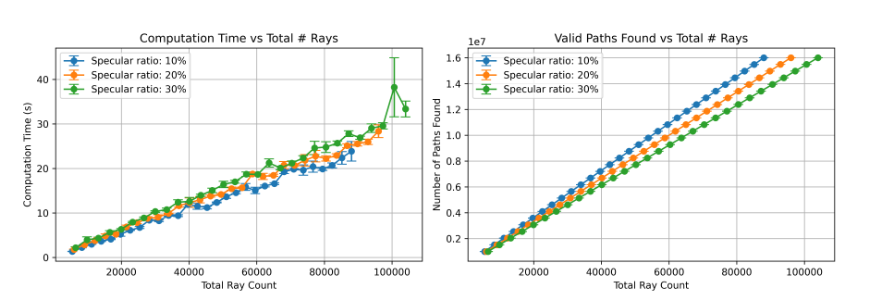
\includegraphics[width=0.75\linewidth]{Figures/gsound_computation_time.png} % Asegúrate de guardar el recorte con este nombre
    \caption[Coste computacional del trazado de rayos]{Relación entre el tiempo de cálculo computacional y el número total de rayos emitidos, categorizado por el porcentaje de rayos especulares. El escalado estrictamente lineal subraya la limitación del método para simulaciones de alta densidad acústica. \cite{Zang2025GSoundSIR}}
    \label{fig:gsound_computation}
\end{figure}
    
    \item \textbf{Sobrecarga por reflexiones especulares:} La validación de trayectorias físicas libres de obstrucciones entre la fuente y el oyente es computacionalmente costosa. Las configuraciones de simulación que exigen un mayor porcentaje de reflexión especular frente a la difusa incrementan exponencialemente el tiempo de cálculo \cite{Zang2025GSoundSIR}.
    
    \begin{figure}[H]
        \centering
        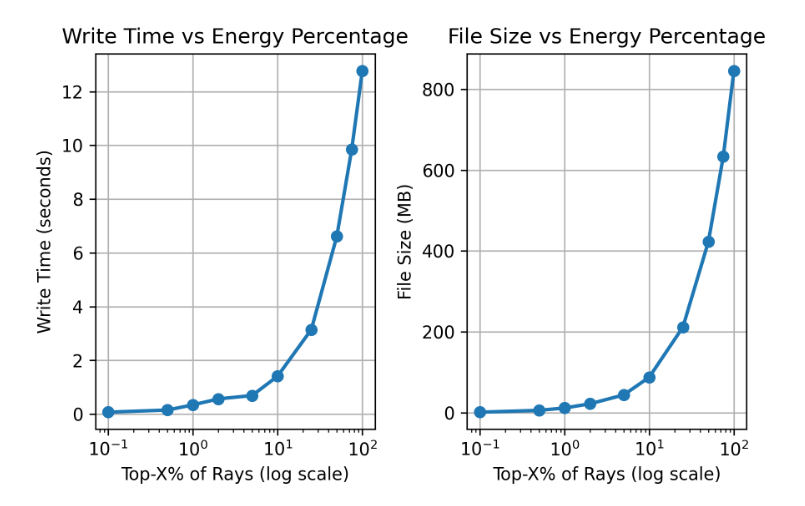
\includegraphics[width=0.85\linewidth]{Figures/gsound_storage_performance.png} % Asegúrate de que el nombre del archivo coincida
        \caption[Rendimiento de almacenamiento según porcentaje de rayos]{Relación entre el tiempo de escritura en disco (izquierda) y el tamaño del archivo resultante (derecha) en función del porcentaje de rayos de mayor energía procesados. Aprovechar la redundancia energética descartando la inmensa mayoría de rayos de baja energía permite un ahorro drástico en los costes de almacenamiento y lectura de la simulación. \cite{Zang2025GSoundSIR}}
        \label{fig:gsound_storage}
    \end{figure}

    
    \item \textbf{Redundancia energética masiva:} El análisis de distribución de energía en simulaciones densas revela que el cálculo exhaustivo de rayos es extremadamente ineficiente. Las mediciones indican que apenas el $0,1\%$ de los rayos capturan el $81,8\%$ de la energía acústica total de la sala, y el $10\%$ superior de los rayos modela el $99,6\%$ de la energía \cite{Zang2025GSoundSIR}. Esto demuestra que los métodos tradicionales invierten la inmensa mayoría de sus ciclos de reloj en trazar decenas de miles de reflexiones tardías que apenas aportan una fracción marginal a la reconstrucción energética de la RIR.
    
    \begin{figure}[H]
    \centering
    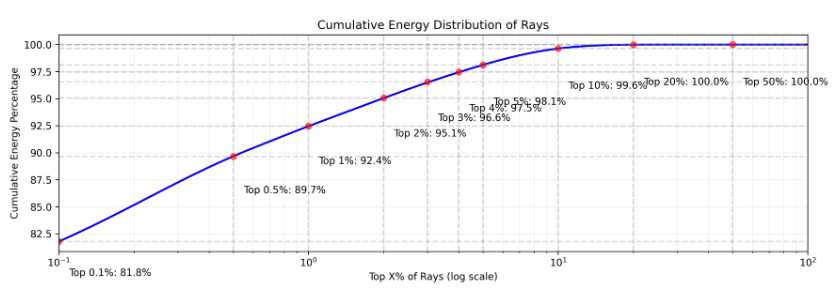
\includegraphics[width=0.75\linewidth]{Figures/gsound_energy_distribution.png} % Asegúrate de guardar el recorte con este nombre
    \caption[Distribución de energía acústica en trazado de rayos]{Distribución de energía acústica acumulada en función del porcentaje de rayos simulados. Se observa que el 10\% de los rayos de mayor intensidad concentran el 99,6\% de la energía total, evidenciando la redundancia del cálculo exhaustivo para la reverberación tardía. \cite{Zang2025GSoundSIR}}
    \label{fig:gsound_energy}
    \end{figure}
    \end{itemize}

Esta redundancia energética y el alto coste computacional asociado a la resolución espacial exhaustiva evidencian el límite tecnológico del \textit{Ray Tracing}. Como sugieren los propios autores del estudio, la enorme concentración de energía en una fracción mínima de rayos abre la puerta a enfoques basados en aprendizaje profundo \cite{Zang2025GSoundSIR}; específicamente, a modelos capaces de reconstruir y extrapolar la respuesta impulsional completa a partir de un conjunto reducido de rayos de alta energía, los cuales corresponden físicamente al campo directo y a las primeras reflexiones \cite{Zang2025GSoundSIR}. 

\subsection{Método de Fuentes Imagen (ISM)}

El Método de Fuentes Imagen (\textit{Image Source Method}, ISM) es una de las técnicas de acústica geométrica más rigurosas para el modelado de reflexiones especulares. Formalizado originalmente por Allen y Berkley en 1979 para recintos de geometría rectangular estricta \cite{Allen1979}, el algoritmo asume que las interacciones de las ondas sonoras con las superficies rígidas se comportan como reflexiones ópticas en espejos. Matemáticamente, cada reflexión se modela sustituyendo la superficie reflectante por una fuente acústica virtual, ubicada en la posición simétrica a la fuente real respecto al plano de la pared.

La RIR en el punto receptor se construye superponiendo la señal directa y las contribuciones retrasadas y atenuadas de todas las fuentes imagen iterativas. Si bien el ISM ofrece una exactitud temporal absoluta para las primeras reflexiones, su viabilidad colapsa rápidamente al incrementar el orden de reflexión necesario para modelar la reverberación tardía. 

La extensión del algoritmo a recintos de topología arbitraria (poliedros), desarrollada por Borish en 1984 \cite{Borish1984}, puso de manifiesto el verdadero cuello de botella de esta metodología: el coste computacional. A diferencia de las geometrías de caja, en geometrías complejas el algoritmo debe realizar costosas pruebas de intersección y validación de visibilidad para garantizar que la trayectoria desde cada fuente virtual hasta el receptor no está obstruida por otros planos del recinto \cite{Borish1984}. 

\begin{figure}[htbp]
\centering
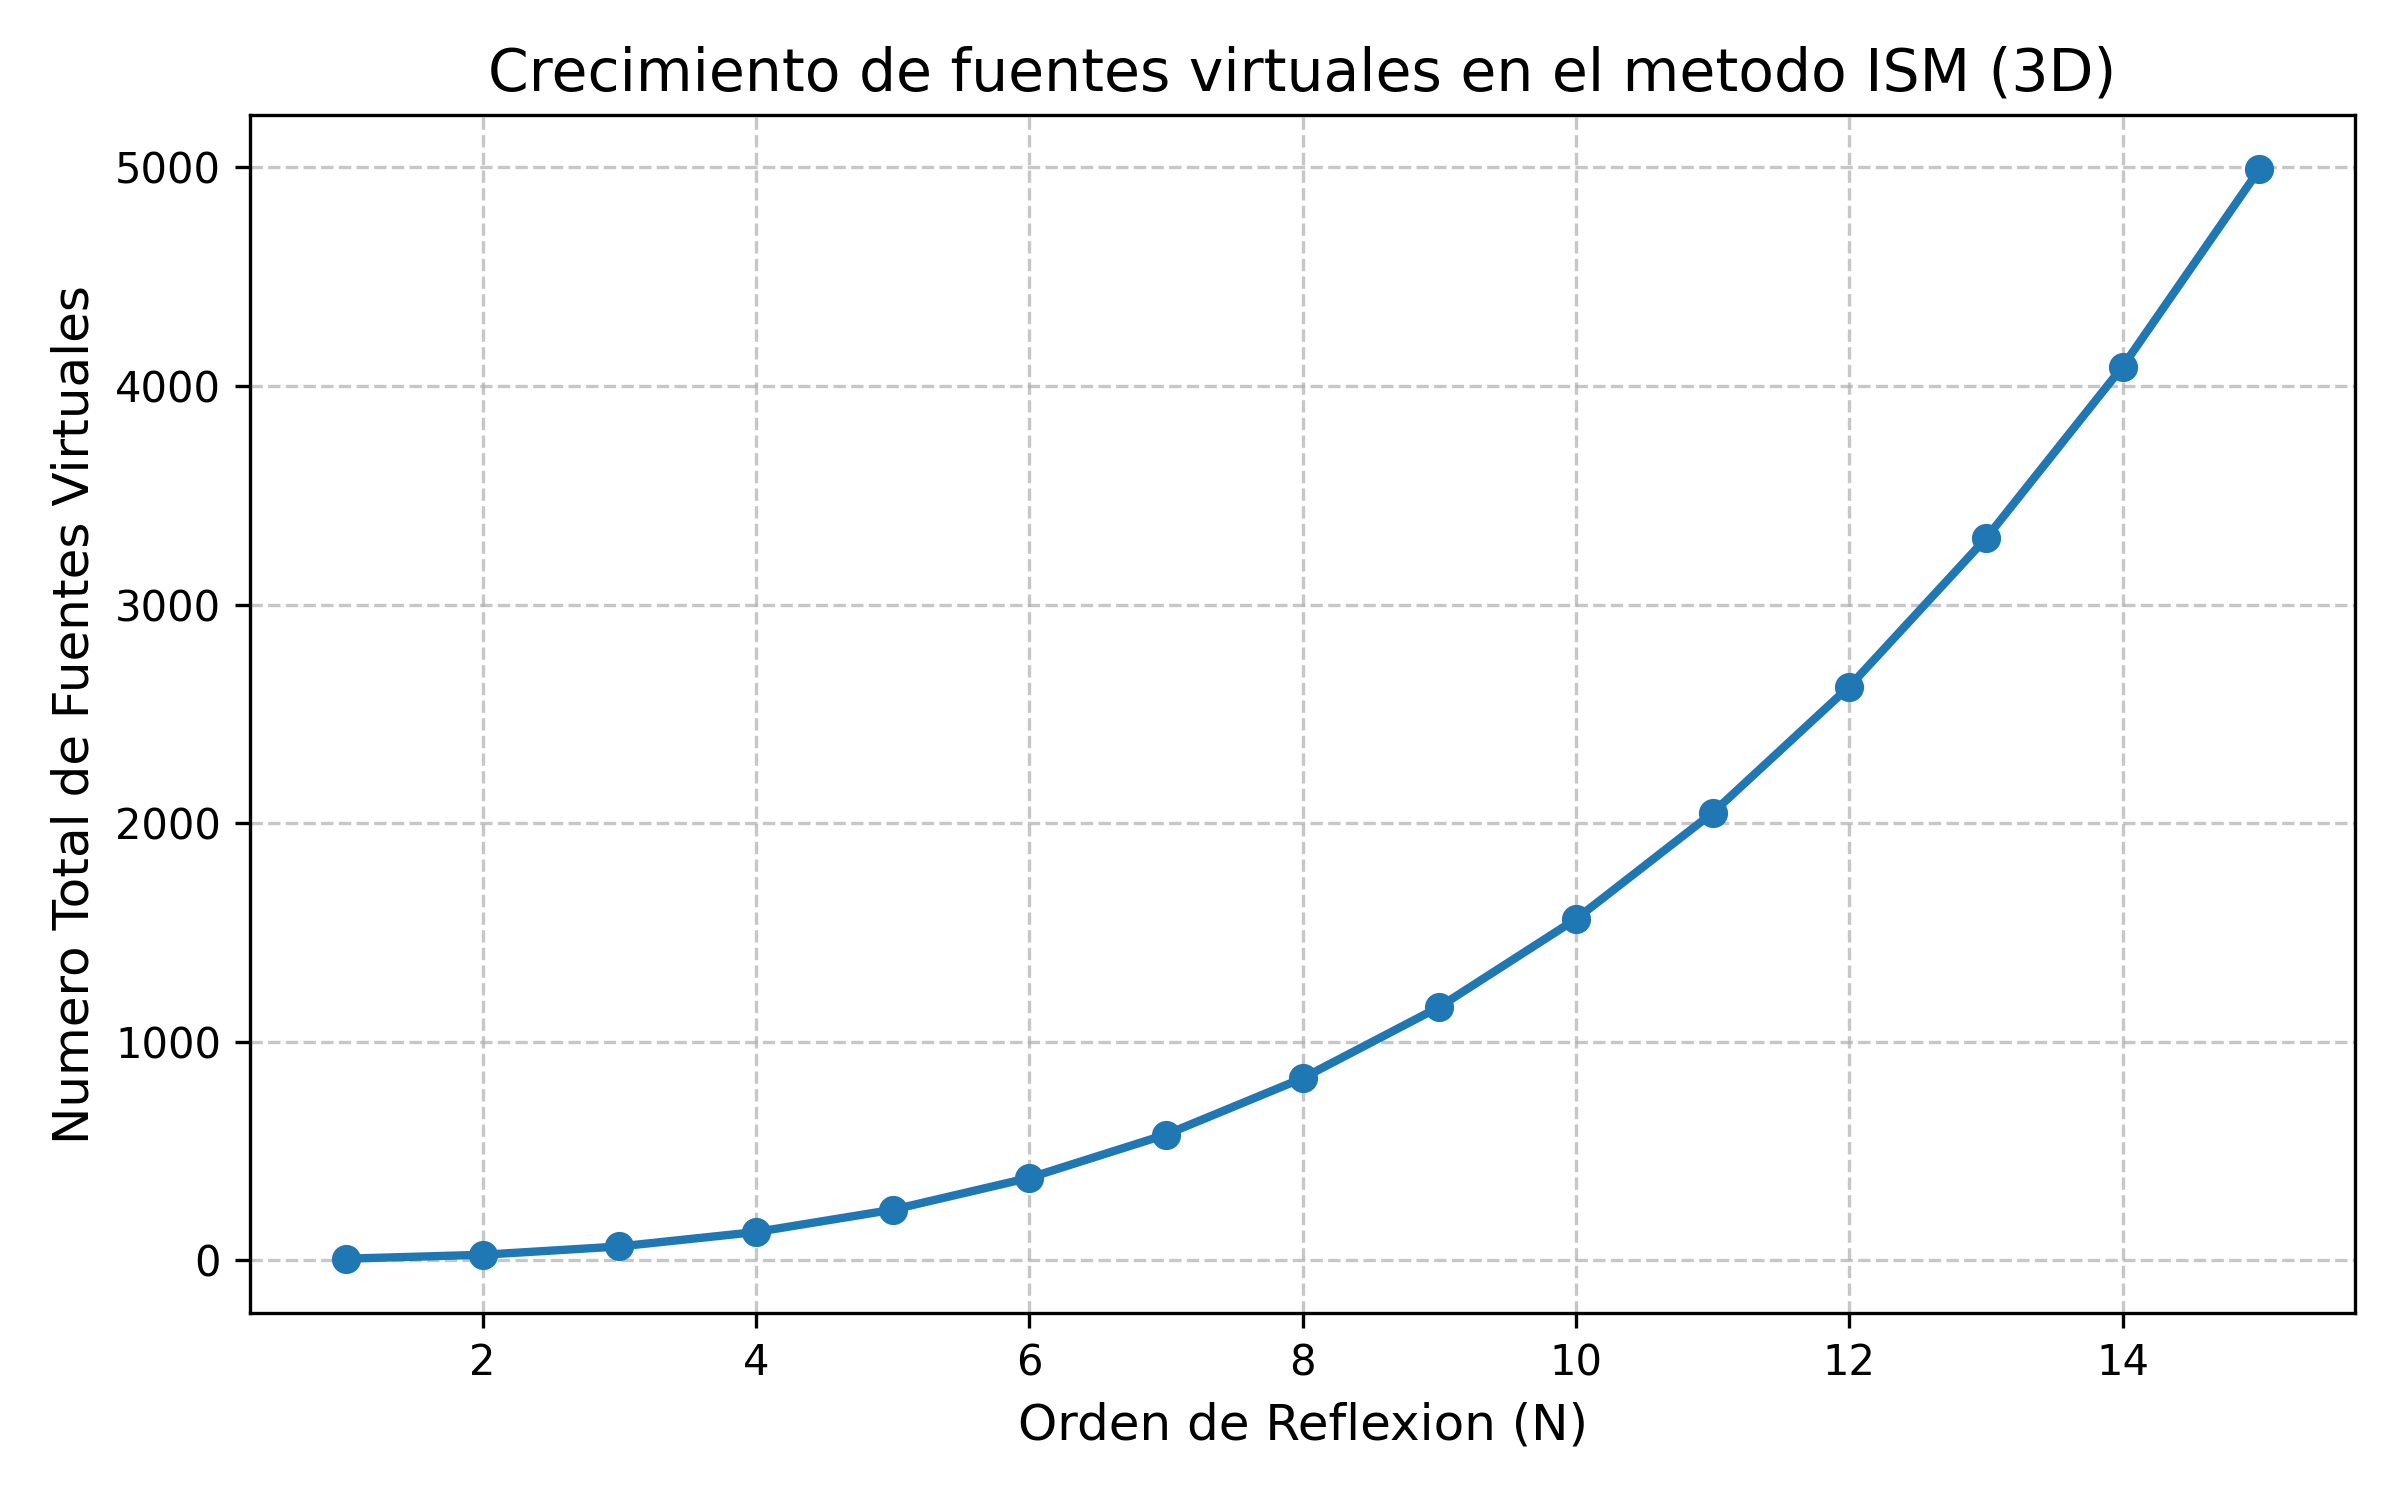
\includegraphics[width=0.8\textwidth]{../Figures/ism_cubic_growth.png}
\caption[Crecimiento cúbico en ISM]{Crecimiento del número de fuentes virtuales en el Método de Fuentes Imagen (ISM) en 3D en función del orden de reflexión $N$. La tendencia muestra un comportamiento polinómico dominante de orden cúbico, coherente con $\mathcal{O}(N^3)$.}
\label{fig:ism_cubic_growth}
\end{figure}

Este esfuerzo de cómputo se agrava drásticamente debido a la naturaleza matemática del propio método. En un espacio tridimensional, el número de fuentes virtuales generadas escala de forma \textbf{cúbica} ($O(N^3)$) con respecto al orden de reflexión $N$. Dado que la densidad de ecos en una sala real aumenta proporcionalmente al cuadrado del tiempo, simular los tramos finales de la curva de decaimiento de energía exige computar un volumen inasumible de fuentes imagen. Por tanto, mientras que el ISM es la herramienta ideal para extraer la firma geométrica inicial del recinto (los primeros milisegundos de la RIR), su crecimiento polinómico de orden tres lo descarta por completo como método autónomo para la síntesis completa de la reverberación.

\section[Aprendizaje profundo]{Enfoques basados en Machine Learning}

\subsection{De la simulación explícita a los modelos predictivos}

\subsection{FiNS: Filtered Noise Shaping}

En el ámbito de la estimación ciega de la respuesta al impulso de la sala (RIR) a partir de voz reverberante, el modelo FiNS (Filtered Noise Shaping) \cite{Steinmetz2021FiNS} propone un enfoque basado en el aprendizaje profundo para la estimación directa en el dominio del tiempo. Este método resulta útil para aplicaciones de realidad aumentada y posproducción de audio, donde se requiere un emparejamiento acústico preciso y de alta fidelidad operando a 48 kHz.

A diferencia de los enfoques que predicen parámetros para reverberadores algorítmicos o emplean modelos de transformación de gran tamaño, FiNS modela directamente la acústica del espacio basándose únicamente en una grabación de referencia. Esto permite reemplazar simulaciones complejas por una operación de convolución simple entre una señal de entrada y la RIR predicha.

Para lograr esto, la arquitectura de la red incorpora un fuerte sesgo inductivo inspirado en la acústica de salas, separando el modelado de la respuesta mediante un codificador y un decodificador especializados. El codificador en el dominio del tiempo procesa la señal de entrada utilizando bloques de convoluciones unidimensionales para capturar el comportamiento temporal a diferentes escalas, generando finalmente un espacio latente. 
   
\begin{figure}[H]
    \centering
    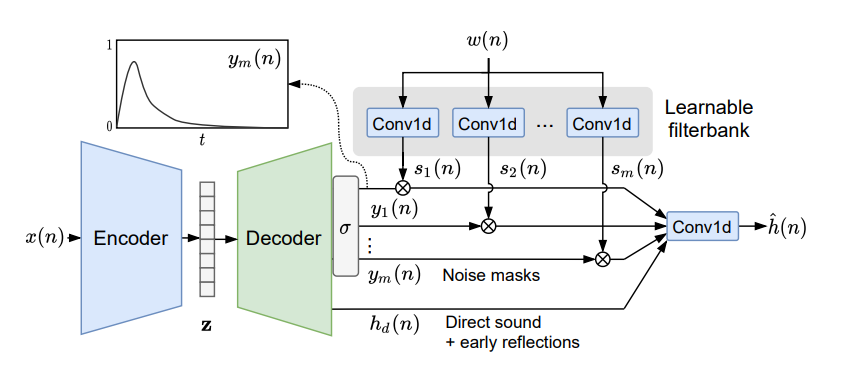
\includegraphics[width=0.8\linewidth]{Figures/arquitecture_Fins.png} % Asegúrate de guardar el recorte con este nombre
    \caption[Arquitectura de FiNS]{Esquema de la arquitectura de FiNS, destacando el codificador temporal y el decodificador especializado para modelar por separado la respuesta temprana (sonido directo y primeras reflexiones) y la reverberación tardía (cola reverberante).\cite{Steinmetz2021FiNS}}
    \label{fig:fins_architecture}
\end{figure}

En la arquitectura propuesta para la síntesis y estimación acústica, el modelo procesa una señal de entrada en el dominio del tiempo $x(n)$ mediante un codificador (\textit{Encoder}) para extraer un vector de características en el espacio latente $\mathbf{z}$. A partir de esta representación, el decodificador (\textit{Decoder}) divide la reconstrucción de la respuesta al impulso de la habitación en dos enfoques complementarios basados en la física del sonido.

Por un lado, estima de manera directa el sonido directo y las reflexiones tempranas, componente denotado como $h_d(n)$. Por otro lado, para modelar la reverberación tardía de naturaleza estocástica, el decodificador genera un conjunto de máscaras de ruido o envolventes temporales $y_1(n), \dots, y_m(n)$ (restringidas al rango de valores entre 0 y 1 mediante una función de activación sigmoide $\sigma$). 

Simultáneamente, una señal de ruido blanco continuo $w(n)$ alimenta un banco de filtros convolucionales unidimensionales entrenable (\textit{Learnable filterbank}), generando múltiples componentes de ruido en subbandas $s_1(n), \dots, s_m(n)$. Cada máscara de ruido proyectada por el decodificador modula en amplitud a su respectiva subbanda de ruido para emular el decaimiento exponencial característico de la energía acústica con el tiempo.

Finalmente, el conjunto de las subbandas moduladas por las envolventes y la componente inicial $h_d(n)$ se combinan e integran a través de una última capa convolucional de una dimensión (Conv1d) para producir la estimación completa y final de la respuesta al impulso de la habitación $\hat{h}(n)$.

El aspecto más destacable para la extrapolación acústica reside en el decodificador, el cual descompone la síntesis de la RIR modelando por separado la respuesta temprana y la cola reverberante. Por un lado, la red utiliza un canal de salida dedicado para predecir directamente en el dominio del tiempo las muestras correspondientes al sonido directo y a las primeras reflexiones.

Por otro lado, la reverberación tardía se modela como una suma de señales de ruido filtrado en decaimiento. Para generar esta cola reverberante, el decodificador produce máscaras temporales que modulan un conjunto de señales de ruido procesadas por un banco de filtros aprendibles.

Esta estrategia de combinar la predicción directa para las componentes tempranas y un enfoque estocástico basado en la conformación de ruido para la parte tardía resulta muy efectiva.

Las evaluaciones demuestran que FiNS no solo es capaz de sintetizar RIRs que coinciden con los parámetros objetivos de la sala, como el tiempo de reverberación ($T_{60}$) y la relación directo-reverberante (DRR), sino que también reproduce las características perceptivas con mayor realismo y precisión que otras arquitecturas base de aprendizaje profundo \cite{Steinmetz2021FiNS}.
\subsection[PINNs]{PINNs: Physics-Informed Neural Networks}

\subsection[DECOR]{DECOR: Deep Exponential Completion Of Room Impulse Responses}

El modelado preciso de la reverberación tardía resulta costoso computacionalmente, pero el sonido directo y las primeras reflexiones encapsulan información suficiente sobre la geometría de la sala y sus características de absorción. Para explotar esta relación, se ha formalizado la tarea de \textit{RIR completion} (completado de la respuesta al impulso de la sala), cuyo objetivo es sintetizar la reverberación tardía a partir de la porción temprana (los primeros 50~ms) de la respuesta \cite{Lin25}.

\begin{figure}[H]
    \centering
    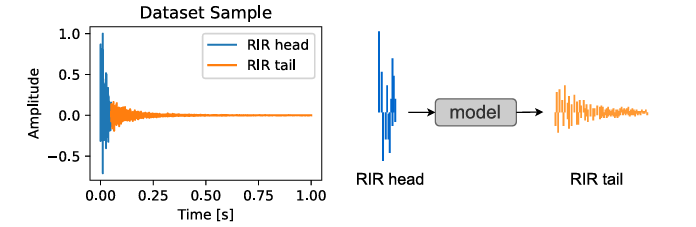
\includegraphics[width=0.68\linewidth]{Figures/rir_completion.png}
    \caption{Concepto de \textit{RIR completion}: extrapolación de la reverberación tardía a partir del tramo temprano de la respuesta al impulso \cite{Lin25}.}
    \label{fig:rir_completion}
\end{figure}


Para abordar este problema, se han propuesto arquitecturas basadas en el paradigma codificador-decodificador (\textit{encoder-decoder}). El modelo DECOR (\textit{Deep Exponential Completion Of Room impulse responses}) es un exponente de esta tendencia \cite{Lin25}. En este sistema, un codificador convolucional temporal profundo comprime la estructura de los primeros 50~ms en un vector latente de baja dimensión de 128 dimensiones. Posteriormente, un decodificador utiliza este vector para parametrizar un modelo físico de decaimiento exponencial \cite{Lin25}. 

\begin{figure}[H]
    \centering
    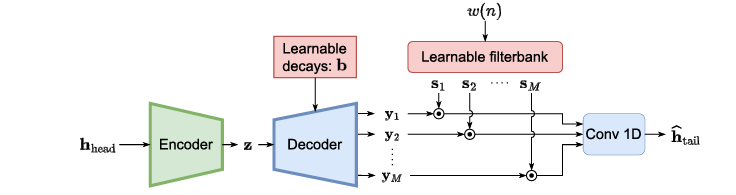
\includegraphics[width=0.75\linewidth]{Figures/encoder-decoder.png}
    \caption{Esquema general de la arquitectura DECOR. El codificador procesa la cabeza de la RIR para generar un vector latente $\mathbf{z}$, que el decodificador utiliza para predecir envolventes de decaimiento aplicadas a un banco de filtros de ruido \cite{Lin25}.}
    \label{fig:decor_overview}
\end{figure}

DECOR se presenta como una evolución conceptual y estructural frente a arquitecturas previas como FiNS (\textit{Filtered Noise Shaping}) \cite{Steinmetz2021FiNS,Lin25}. FiNS fue diseñado originalmente para una tarea de estimación ciega, tomando fragmentos de varios segundos de voz reverberante para predecir la RIR \cite{Steinmetz2021FiNS}. Aunque DECOR adapta la estructura del codificador de FiNS mediante convoluciones unidimensionales y conexiones residuales, la diferencia fundamental entre ambas redes radica en el diseño de su decodificador y en la imposición de un fuerte sesgo inductivo basado en la acústica de salas para la síntesis de la reverberación tardía \cite{Lin25}.

Mientras que el decodificador de FiNS utiliza un enfoque basado en sobremuestreo convolucional (\textit{convolution upsampling}) \cite{Steinmetz2021FiNS}, DECOR modela estocásticamente la reverberación tardía como ruido blanco moldeado por una suma de envolventes de decaimiento exponencial \cite{Lin25}. Específicamente, el decodificador de DECOR emplea un perceptrón multicapa (MLP) que toma el vector latente y predice matrices de amplitud temporal. Estas amplitudes se multiplican por tasas de decaimiento aprendibles (inicializadas para decaimientos $T_{60}$ entre 0.05 y 3.0 segundos) para formar envolventes que modulan secuencias de ruido generadas por un banco de filtros de respuesta finita (FIR) en bandas de octava \cite{Lin25}.

Esta reformulación arquitectónica aporta ventajas significativas frente a FiNS que justifican su adopción para el completado de RIRs:

\begin{itemize}
    \item \textbf{Eficiencia computacional y tamaño del modelo:} La parametrización física en el decodificador permite que DECOR sea extremadamente ligero. El modelo DECOR ocupa únicamente 37~MB, lo que lo hace más de 30 veces más pequeño que la arquitectura base de FiNS, cuyo peso asciende a 1,3~GB \cite{Lin25}. Esta reducción drástica de parámetros facilita su despliegue en aplicaciones de síntesis en tiempo real para entornos dinámicos de realidad virtual o aumentada.
    
    \item \textbf{Eliminación de artefactos acústicos:} Las redes generativas que no imponen restricciones físicas estrictas sobre la síntesis de la señal suelen presentar problemas perceptuales. FiNS tiende a generar picos dispersos de gran amplitud en la cola de la RIR, lo que introduce una "granulosidad" (\textit{graininess}) poco natural en el audio resultante \cite{Steinmetz2021FiNS,Lin25}. Al forzar a la red a predecir parámetros para un modelo de decaimiento exponencial puro, DECOR garantiza curvas de decaimiento suaves y un sonido más realista y coherente con el comportamiento acústico natural \cite{Lin25}.
    
    \item \textbf{Mejora en métricas objetivas:} DECOR supera a FiNS en la evaluación de la similitud con las características acústicas de la sala objetivo. Logra reducir el error en el dominio espectro-temporal (MSTFT), mejora la precisión de la función de decaimiento de energía (EDF), y estima con mayor exactitud tanto el tiempo de reverberación ($T_{60}$) como la relación directo-reverberante (DRR) \cite{Lin25}. 
    
    \item \textbf{Capacidad de generalización:} Aunque la extrapolación de una señal a veinte veces su longitud original es una tarea compleja que penaliza a ambos modelos ante datos no vistos, DECOR mantiene un mejor rendimiento de generalización. Frente a conjuntos de datos de medición reales que la red no ha observado durante el entrenamiento, DECOR sigue siendo capaz de deducir relaciones correctas del $T_{60}$ y superar a FiNS, demostrando que su arquitectura de decaimiento estructurado es más robusta frente a escenarios acústicos fuera de distribución \cite{Lin25}.
\end{itemize}

En conclusión, la transición de un enfoque de sobremuestreo genérico a un modelo fuertemente condicionado por la física acústica permite que DECOR resuelva el problema del \textit{RIR completion} de forma mucho más eficiente. La parametrización directa de variables como el decaimiento por bandas de octava no solo elimina la inestabilidad de las muestras individuales, sino que dota a la red de una alta expresividad para modelar escenarios acústicos complejos manteniendo una huella computacional mínima. Por este motivo, DECOR constituye el método seleccionado para ser implementado y empleado en el desarrollo de este trabajo.


\newpage

\chapter[Planteamiento]{Planteamiento y decisión sobre las soluciones alternativas}

La etapa de diseño del sistema DECOR requirió evaluar varias alternativas arquitectónicas antes de fijar la solución definitiva. En este capítulo se describen las opciones consideradas para cada componente del sistema y se justifica la elección adoptada.

\section[Alternativas para la extrapolación]{Alternativas para la extrapolación de la reverberación tardía}

La cola de una RIR comparte tres características físicas universales: decaimiento exponencial, coloración espectral dependiente de los materiales y un componente estocástico de alta frecuencia. Esto abre dos familias de enfoques:

\begin{itemize}
	\item \textbf{Regresión directa de la señal temporal:} El modelo predice directamente las muestras de audio. Permite el uso de cualquier función de pérdida temporal o espectral, pero supone un objetivo de alta dimensionalidad (48000 muestras) con elevada varianza aleatoria, haciendo el aprendizaje inestable.
	\item \textbf{Modelo físico paramétrico:} El modelo predice parámetros de un modelo analítico de decaimiento (p. ej., coeficientes de decaimiento exponencial por banda de octava) que luego sintetizan la señal. Reduce el espacio de salida a unas pocas decenas de números, garantizando plausibilidad física por construcción.
\end{itemize}

Se optó por el \textbf{modelo físico paramétrico} por su estabilidad durante el entrenamiento y su interpretabilidad, siguiendo el marco propuesto en \cite{muhammad2025}.

\section[Alternativas para el codificador]{Alternativas para el codificador de la cabeza}

Para extraer el vector latente a partir de los primeros 50~ms de la RIR se consideraron tres arquitecturas:

\begin{table}[H]
	\centering
	\caption{Comparativa de arquitecturas de codificador consideradas}
	\begin{tabular}{|p{3cm}|p{5cm}|p{5cm}|}
		\hline
		\textbf{Arquitectura} & \textbf{Ventajas} & \textbf{Inconvenientes} \\ \hline
		LSTM bidireccional & Modela dependencias temporales nativas & Secuencial, difícil de paralelizar; costoso en señales largas \\ \hline
		Transformer & Atención global, altamente paralelizable & Coste cuadrático en longitud de secuencia sin optimizaciones \\ \hline
		CNN residual (elegida) & Paralelizable, campo receptivo controlado, estable con BN & Requiere un número elevado de bloques para cubrir toda la cabeza \\ \hline
	\end{tabular}
\end{table}

Se eligió la \textbf{CNN residual con stride} (\texttt{DecorEncoder}) porque combina campo receptivo suficientemente amplio ($>100.000$ muestras con 14 bloques de stride 2), paralelización completa en GPU y estabilidad de entrenamiento gracias a \textit{BatchNorm} y conexiones residuales.

\section{Alternativas para la función de pérdida}

La pérdida es un factor crítico para la calidad perceptual. Las alternativas estudiadas fueron:

\begin{itemize}
	\item \textbf{MSE en tiempo:} Simple pero ciega a la percepción espectral; penaliza errores de fase irrelevantes perceptualmente.
	\item \textbf{MAE en EDC:} Favorece la corrección de la envolvente energética; no penaliza errores espectrales de coloración.
	\item \textbf{MSTFT (elegida):} Combina pérdida de convergencia espectral y pérdida de log-magnitud en cuatro resoluciones temporales/frecuenciales, siendo la más alineada con la percepción humana y con el estado del arte \cite{Lin25}.
\end{itemize}

La implementación final (\texttt{models/loss.py}) utiliza resoluciones FFT de $\{64, 512, 2048, 8192\}$ con saltos $\{32, 256, 1024, 4096\}$, cubriendo desde detalles de ataque hasta la macro-envolvente del decaimiento.

\section{Decisión sobre el dataset de entrenamiento}

Se evaluaron dos fuentes de datos:

\begin{enumerate}
	\item \textbf{Dataset sintético propio:} 6000 salas rectangulares generadas con Pyroomacoustics (ISM). Ventaja: configuración controlada, trazabilidad total. Inconveniente: distribución acotada a geometrías simples.
	\item \textbf{BIRD \cite{Grondin25}:} Dataset real con 89 splits y miles de RIR medidas en recintos reales de todo tipo. Mayor diversidad geométrica y de materiales.
\end{enumerate}

Se adoptó \textbf{BIRD como fuente principal} de entrenamiento por su diversidad, reservando el dataset sintético para estudios de ablación y validación de la pipeline de datos.
\newpage

% !TeX root = ../main.tex

\chapter{Marco Experimental y Datasets}

Este capítulo expone el marco metodológico y experimental  para la aplicación y evaluación de la arquitectura propuesta. En primer lugar, se describe el conjunto de datos empleado como base de aprendizaje del modelo, detallando el preprocesamiento del corpus masivo BIRD. A continuación, se define la cadena de procesamiento de la señal, centrada en el cálculo de la Curva de Decaimiento de Energía (EDC) para el correcto acondicionamiento y análisis de las respuestas acústicas. Finalmente, se detalla la fase de entrenamiento, estableciendo las estrategias de optimización y los criterios de evaluación que permiten cuantificar el rendimiento y la capacidad de generalización de la red neuronal.

\section{Corpus BIRD}

El \textit{Big Impulse Response Dataset} (BIRD) \cite{Grondin25} constituye la fuente principal de datos empleada en este trabajo para el entrenamiento y validación de la arquitectura DECOR. En su concepción original, este conjunto de datos se define como el mayor corpus abierto de respuestas al impulso en salas multicanal, compuesto por un total de 100.000 RIRs simuladas mediante el Método de la Imagen (\textit{Image Method}). Sin embargo, para los experimentos desarrollados en esta investigación, se ha seleccionado un subconjunto representativo de 40.000 respuestas. Esta dimensión muestral mantiene una base estadística suficientemente robusta para el entrenamiento de la red neuronal, a la vez que optimiza el coste computacional y los tiempos de iteración del modelo. 

El uso de este corpus presenta ventajas sustanciales para la tarea que nos ocupa. Cada simulación varía aleatoriamente parámetros clave como las dimensiones físicas de la sala, la velocidad del sonido y las posiciones relativas de 2 micrófonos y 4 fuentes de sonido omnidireccionales. Dado que el coste computacional espacial del Método de la Imagen escala de forma cúbica en el espacio tridimensional, disponer de un corpus precalculado de esta magnitud resulta fundamental para agilizar la experimentación.

\begin{figure}[htbp]
    \centering
    % Ajusta el valor 0.7 según lo grande que quieras que se vea en el PDF
    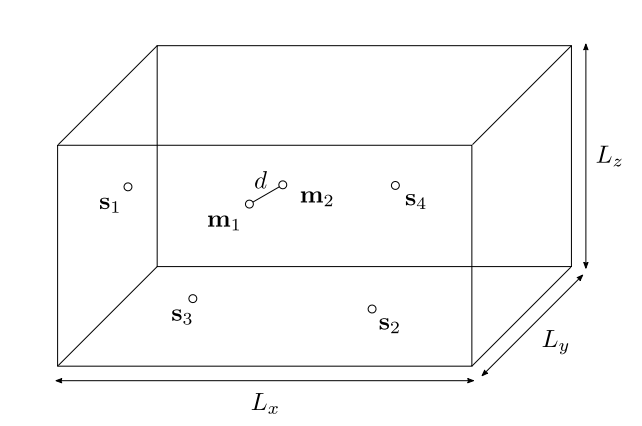
\includegraphics[width=0.7\textwidth]{Figures/bird.png}
    \caption[Configuración espacial BIRD]{Configuración espacial empleada para las simulaciones del corpus BIRD. El entorno virtual consiste en una sala rectangular de dimensiones $L_x \times L_y \times L_z$ metros, en la que se posicionan de manera aleatoria cuatro fuentes de sonido omnidireccionales ($\mathbf{s}_1, \mathbf{s}_2, \mathbf{s}_3, \mathbf{s}_4$) y un par de micrófonos ($\mathbf{m}_1, \mathbf{m}_2$) separados por una distancia $d$ \cite{Grondin25}.}
    \label{fig:bird_setup}
\end{figure}

No obstante, la utilización de BIRD para la extrapolación de la cola reverberante conlleva limitaciones inherentes a su naturaleza sintética que es crucial documentar. La topología del corpus representa una abstracción espacial simplificada: el algoritmo de simulación genera exclusivamente habitaciones vacías estrictamente rectangulares. En BIRD, la absorción de materiales no se modifica en sus RIRs: dentro de una misma sala se emplea un único coeficiente de absorción ($\alpha$) idéntico para todas las superficies (suelo, techo y paredes). 

Esta simplificación ignora la heterogeneidad de materiales presentes en entornos reales, lo que limita la variabilidad frecuencial y direccional de las reflexiones tardías que la red debe aprender a completar.  Desde el punto de vista operativo, los archivos de audio originales—generados a una frecuencia de muestreo nativa de 16 kHz y con 1 segundo exacto de duración (16.000 muestras)—son sometidos a una secuencia estricta de adecuación previa a su paso por la red neuronal. 

En primer lugar, cada señal multicanal se transforma a formato monoaural y se remuestrea a una frecuencia uniforme de 48 kHz, garantizando así la compatibilidad dimensional con la arquitectura DECOR. Sobre esta nueva base temporal, la respuesta se normaliza en amplitud y se alinea con respecto a su pico máximo para asegurar que el transitorio del sonido directo ocupe un índice determinista. Finalmente, la secuencia se ajusta a una longitud fija de 48.000 muestras (equivalentes a 1 segundo exacto).

Una vez acondicionada la señal, se procede a su segmentación en dos regiones de interés. Aprovechando la resolución obtenida tras el remuestreo, se aísla una cabeza temprana de longitud $N_{head} = 2400$ muestras (correspondientes exactamente a los primeros 50 ms), la cual abarca el sonido directo y las reflexiones tempranas. El resto de la secuencia conforma la cola reverberante remanente, que constituye el proceso de decaimiento tardío que el sistema debe aprender a extrapolar. 

\begin{figure}[htbp]
    \centering
    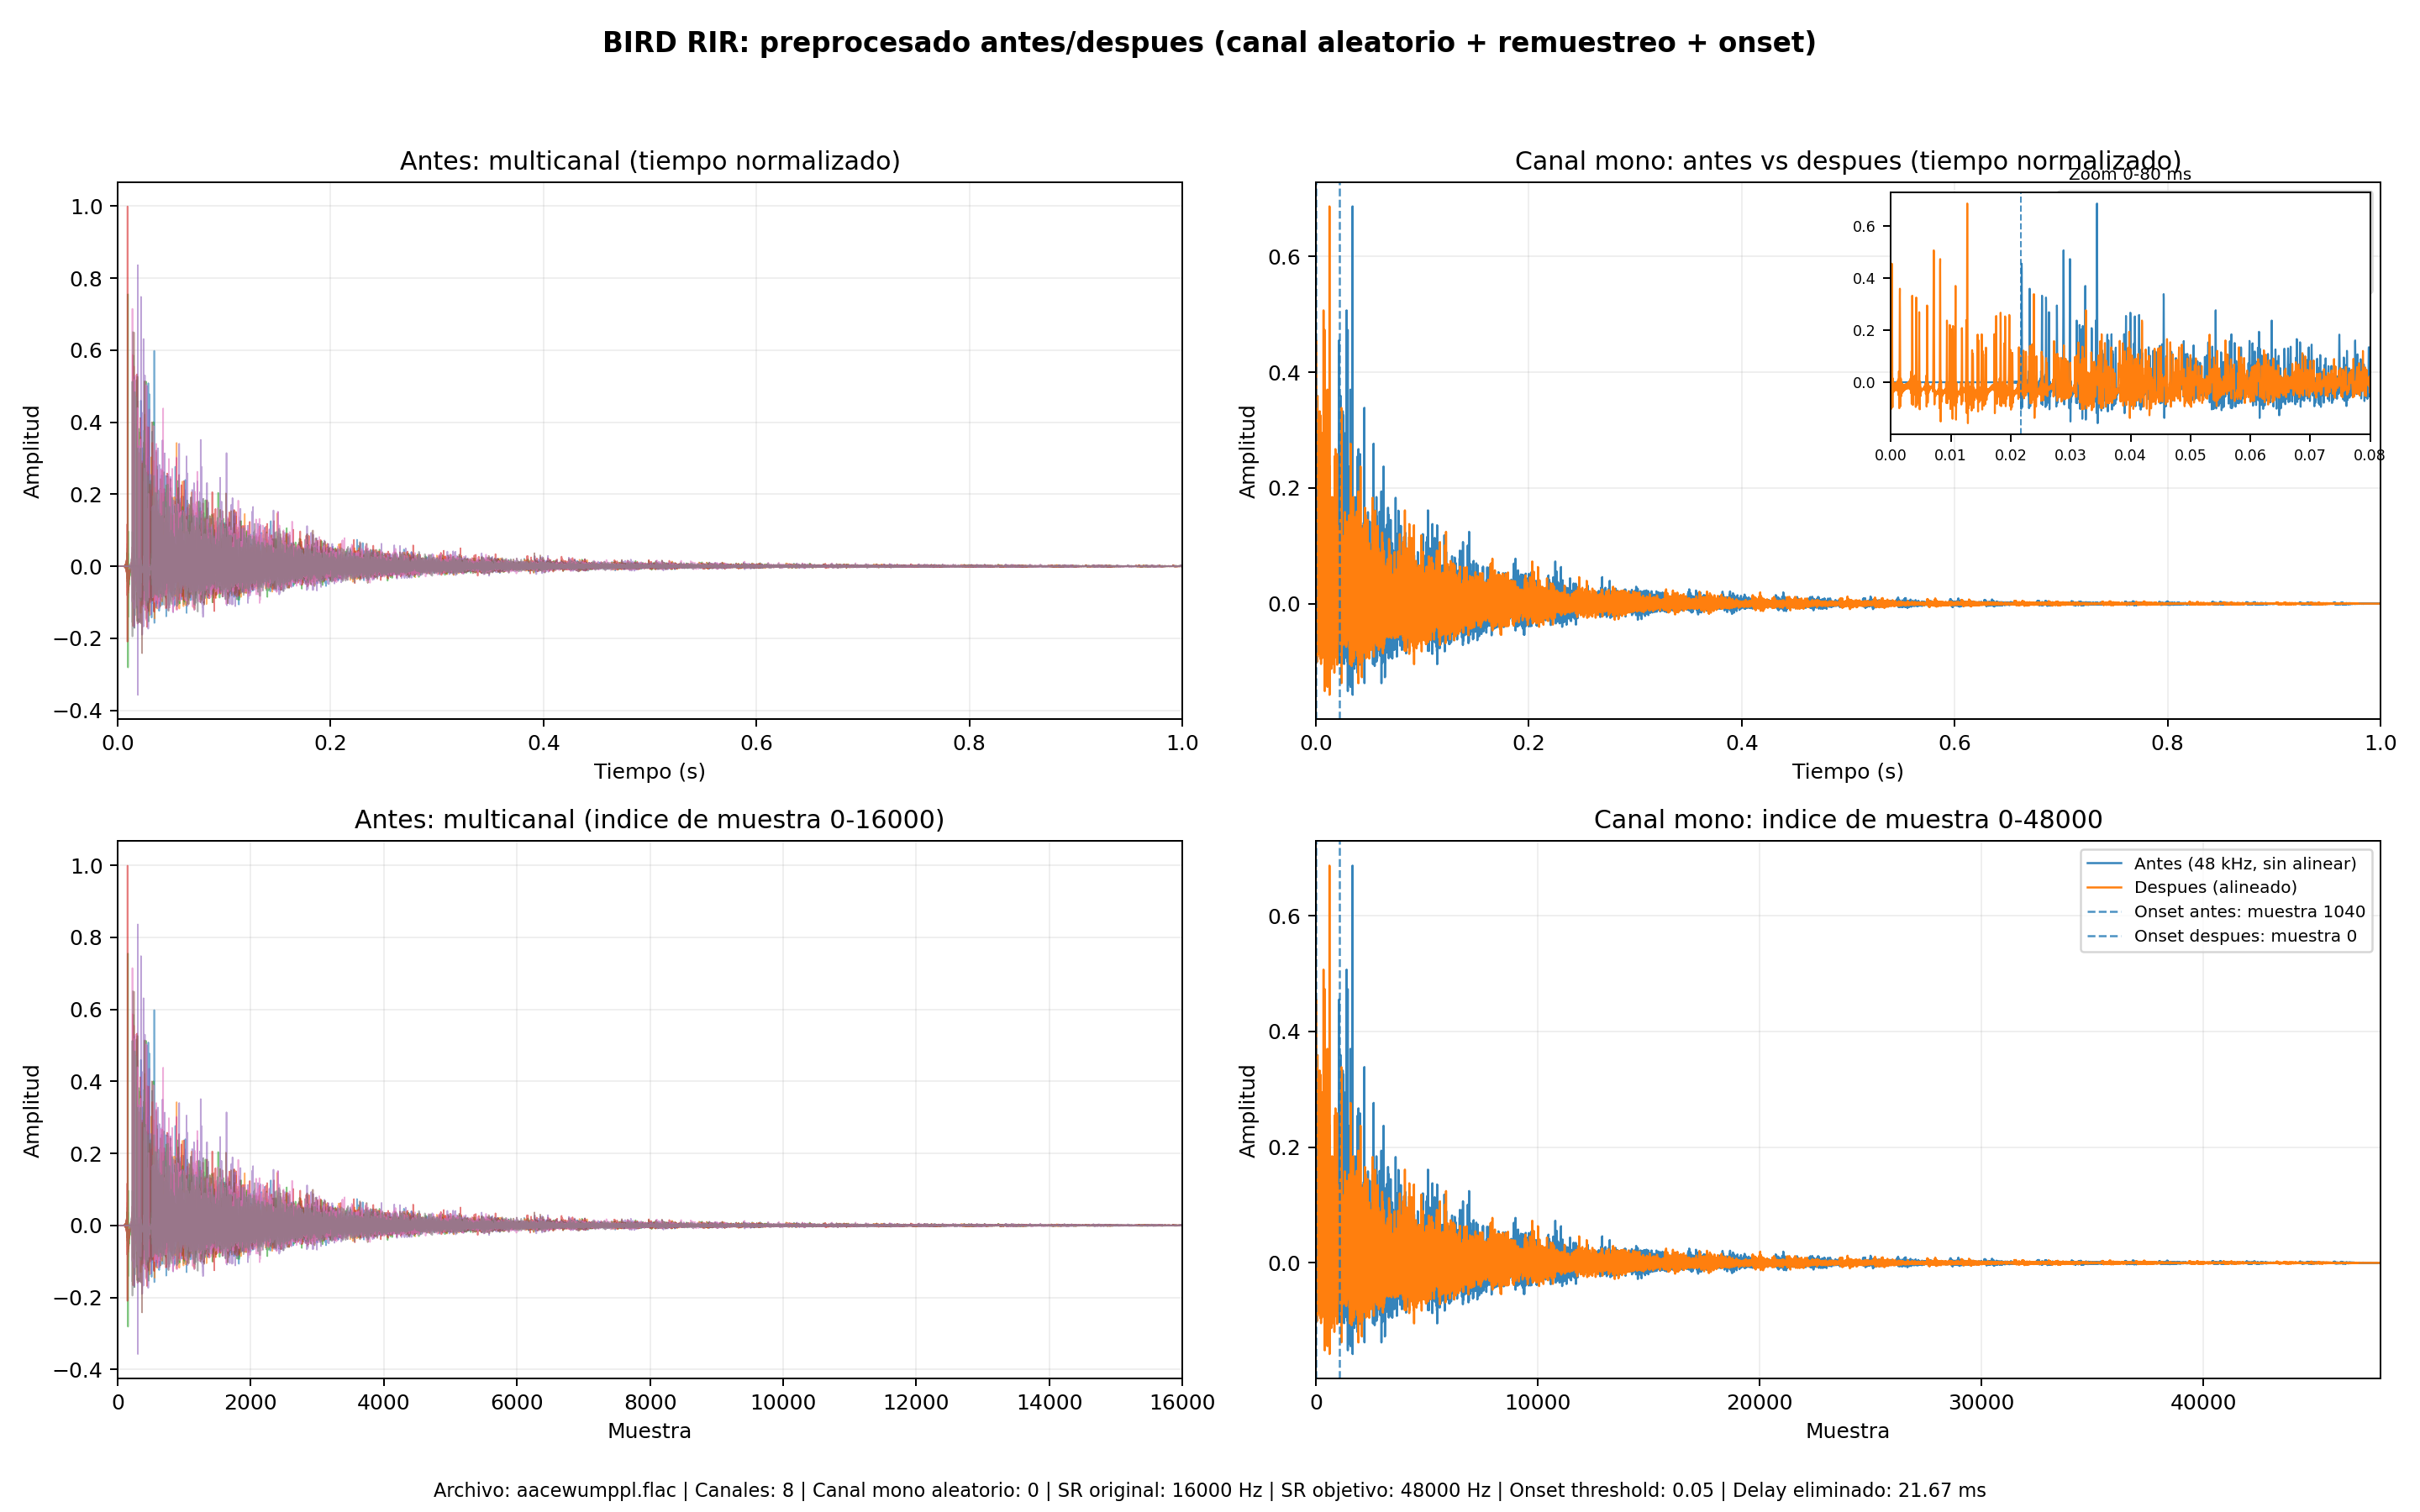
\includegraphics[width=1\textwidth]{Figures/bird_preprocess_before_after_onset.png}
    \caption[Preprocesado BIRD]{Efecto de la etapa de preprocesado sobre una respuesta al impulso del corpus BIRD. El procedimiento ilustrado incluye la extracción de un canal monoaural aleatorio, el sobremuestreo a 48 kHz y la alineación temporal basada en la detección de inicio (\textit{onset detection}). Este método elimina el tiempo de vuelo originado en la simulación preservando la integridad morfológica del sonido directo y de las reflexiones tempranas previas al pico de máxima amplitud.}
    \label{fig:bird_preprocessing_onset}
\end{figure}

Finalmente, para prevenir la contaminación cruzada y el solapamiento acústico, la división del subconjunto de 40.000 respuestas impulsionales entre las fases de entrenamiento y validación no se efectúa de manera aleatoria a nivel de impulso individual, sino aprovechando la estructura de bloques independientes (\textit{folds}) del corpus original. Al establecer la separación mediante estas agrupaciones de salas no solapadas, se garantiza que la evaluación se lleve a cabo sobre recintos acústicos no observados durante el ajuste de pesos, lo que proporciona una estimación rigurosa y fiable de la capacidad de generalización del modelo. 

En resumen, el corpus BIRD ofrece un entorno de simulación controlado y de gran escala para el entrenamiento de modelos de aprendizaje profundo en tareas de extrapolación temporal de RIR. Sin embargo, su naturaleza simulada y sus simplificaciones acústicas introducen limitaciones que deben ser consideradas al interpretar los resultados y extrapolar las conclusiones hacia escenarios del mundo real.

\section{Naive Baseline}

Para evaluar el rendimiento de nuestro modelo y entender el valor real de las métricas obtenidas, es fundamental contar con un punto de referencia básico o línea base. Con este propósito, implementamos un \textit{naive baseline} (o línea base ingenua), que consiste en una aproximación estocástica fija basada puramente en la media estadística del conjunto de datos.

\subsection*{Construcción de la Señal}
Este modelo de referencia no utiliza redes neuronales ni intenta extraer información de los primeros 50 ms del \textit{RIR head}. En su lugar, genera una única cola reverberante genérica combinando ruido blanco con una envolvente de decaimiento exponencial analítica. 

Los parámetros de esta señal (duración, energía y tiempo de reverberación) se configuran de forma estática utilizando los valores promedio de todo el conjunto de entrenamiento. Específicamente, se calibra para que coincida con el $T_{60}$ medio del \textit{dataset}, que en este trabajo es de 0.65 segundos. Posteriormente, esta misma señal fija se evalúa contra todos los RIR reales del conjunto de test para calcular sus métricas de error.

\subsection*{Formulación Matemática}
Matemáticamente, la señal del \textit{naive baseline} en el dominio temporal discreto se define mediante la siguiente ecuación:

\begin{equation}
    h_{\mathrm{naive}}(n) = w(n) \cdot e^{-\gamma n / f_s}
\end{equation}

Donde:
\begin{itemize}
    \item $h_{\mathrm{naive}}(n)$ es la respuesta al impulso calculada para la cola tardía.
    \item $w(n)$ es una secuencia de ruido blanco gaussiano que simula la densidad estocástica de las reflexiones.
    \item $f_s$ es la frecuencia de muestreo (en este trabajo, $f_s=48\,\mathrm{kHz}$).
    \item $\gamma$ es la tasa de decaimiento constante, la cual se vincula directamente al tiempo de reverberación promedio del conjunto de datos ($T_{60,\mathrm{mean}} = 0.65$ s) mediante la relación de atenuación de 60 dB:
    \begin{equation}
        \gamma = \frac{\ln(10^3)}{T_{60,\mathrm{mean}}} \approx \frac{6.91}{T_{60,\mathrm{mean}}}
    \end{equation}
\end{itemize}

\subsection*{Utilidad y Justificación en el Trabajo}
La inclusión de este caso de control es importante en el empleo de nuestro trabajo por tres motivos principales:

\begin{enumerate}
    \item \textbf{Establecer un límite inferior :} Nos da el peor escenario aceptable. Cualquier modelo de aprendizaje profundo que diseñemos debe superar  los resultados de esta aproximación matemática simple para justificar su complejidad computacional.
    \item \textbf{Validar el comportamiento de la red:} Si el modelo DECOR obtiene errores significativamente menores que el \textit{naive baseline}, queda demostrado estadísticamente que la red no se está limitando a devolver la media estocástica de las salas que ha visto durante el entrenamiento, sino que extrae características acústicas específicas del \textit{head} de 50 ms.
    \item \textbf{Contextualizar la escala de los errores:} Nos ayuda a interpretar físicamente las magnitudes de evaluación. Al comparar nuestros resultados frente a la desviación de la media, podemos cuantificar con precisión el porcentaje de mejora del sistema propuesto.
\end{enumerate}
\section{Pipeline EDC}

Dentro del flujo de procesamiento de datos, el cálculo de la Curva de Decaimiento de Energía (EDC, por sus siglas en inglés) se establece como métrica fundamental para evaluar la coherencia del decaimiento reverberante. Dado que la respuesta al impulso tardía presenta un comportamiento altamente estocástico, resulta inviable predecir su forma de onda exacta. Por ello, la EDC permite extraer una envolvente energética determinista que el modelo sí puede aprender a extrapolar. Para una secuencia discreta de la cola reverberante $y[n]$ de longitud $N$, se emplea la forma de integración discreta propuesta originalmente por Schroeder \cite{Schroeder1965}:

\begin{equation}
\mathrm{EDC}_{norm}[t] = \frac{\sum_{n=t}^{N-1} y[n]^2}{\sum_{n=0}^{N-1} y[n]^2}
\end{equation}

En esta formulación, donde $y[n]$ representa la secuencia discreta de la cola reverberante, la EDC se normaliza por la energía total de la cola para garantizar que su valor inicial sea exactamente 1 (0 dB) y que tienda asintóticamente a 0 a medida que el tiempo avanza. Esta normalización es crucial para establecer una escala de análisis coherente y para facilitar la comparación entre diferentes muestras con niveles de energía variables, garantizando una trayectoria monótona decreciente acotada en el intervalo $[0,1]$, con valor unitario al inicio del decaimiento y aproximación asintótica a cero para tiempos tardíos.

Con el fin de obtener una escala de análisis perceptualmente adecuada, la curva normalizada se expresa en decibelios mediante transformación logarítmica:

\begin{equation}
\mathrm{EDC}_{dB}[t] = 10 \log_{10}\left( \max(\mathrm{EDC}_{norm}[t], \epsilon) \right)
\end{equation}

\begin{figure}[htbp]
    \centering
    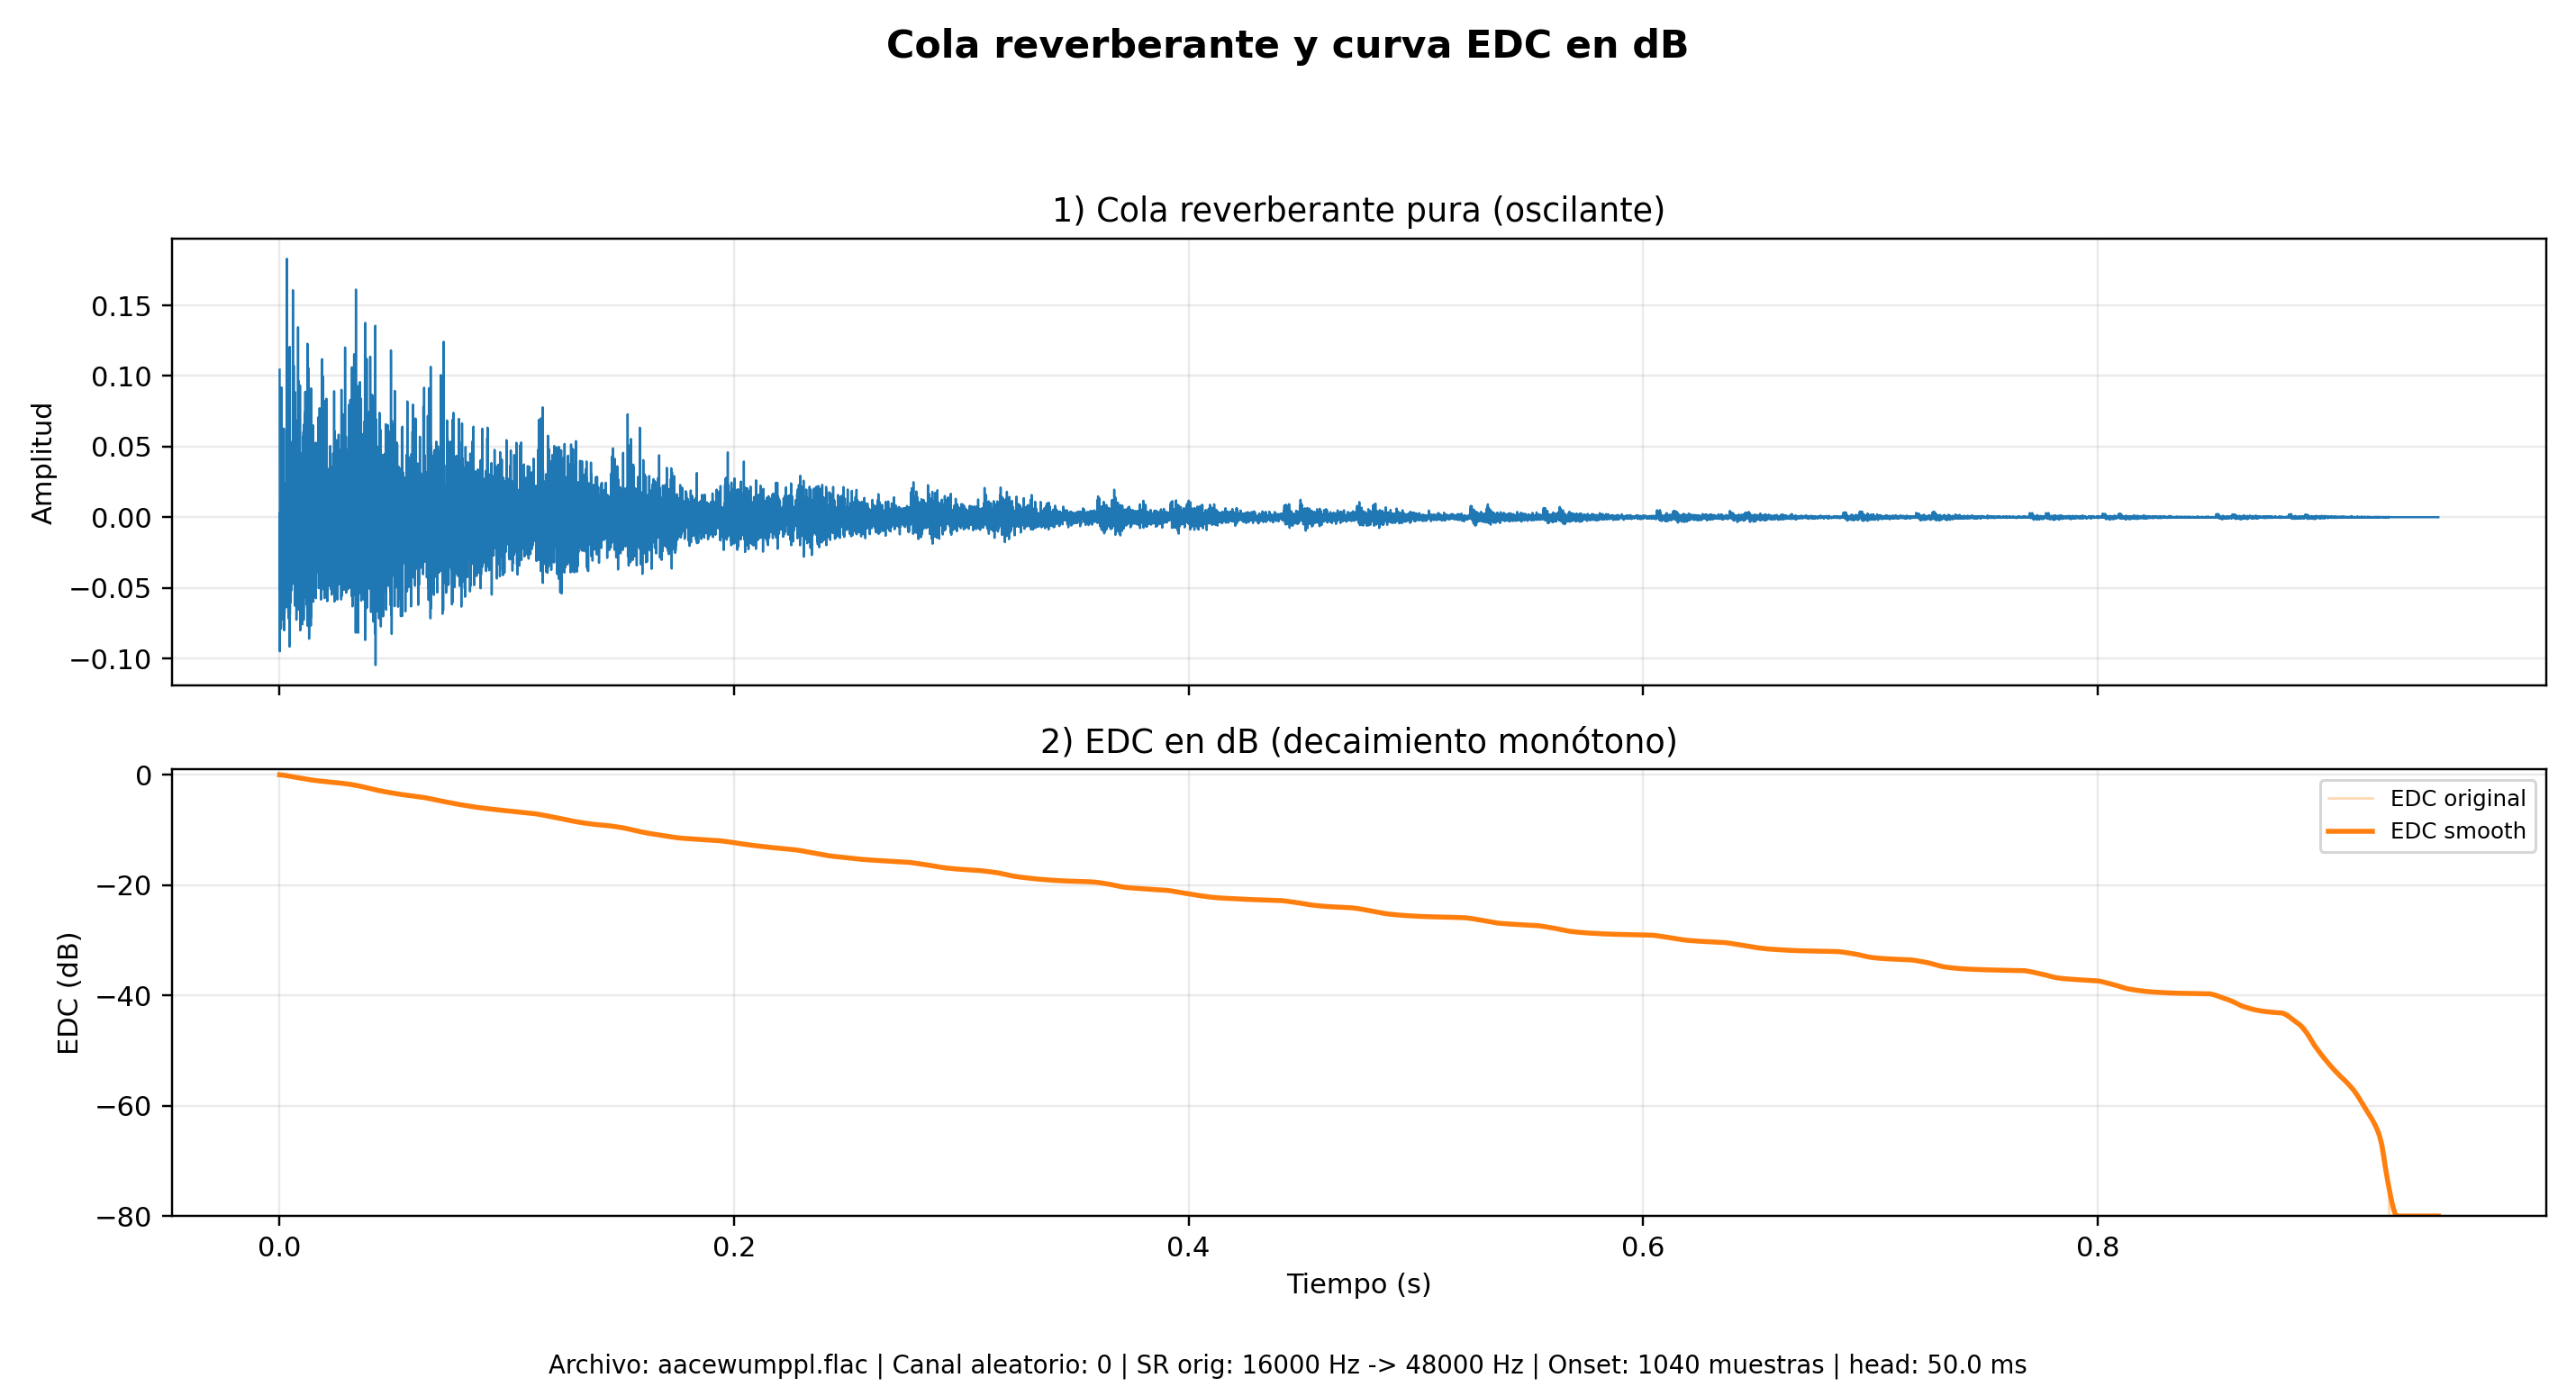
\includegraphics[width=0.8\textwidth]{Figures/tail_edc_overlay.png}
    \caption[Curva de Decaimiento de Energía (EDC) ]{Comparativa visual entre la forma de onda estocástica de una cola reverberante y su correspondiente Curva de Decaimiento de Energía (EDC) expresada en decibelios. Se observa cómo la integración de Schroeder extrae una envolvente energética determinista y monótonamente decreciente, transformando la señal bruta en un objetivo de aprendizaje estable para el modelo predictivo.}
    \label{fig:edc_schroeder}
\end{figure} 

El término de protección $\epsilon$, asociado en práctica a un suelo dinámico del orden de -80 dB, resulta indispensable para preservar estabilidad numérica en el cálculo tensorial, evitando singularidades cuando la energía remanente tiende a cero.

Desde la perspectiva computacional, la lógica de segmentación temporal (corte exacto en la muestra 2400) y el cálculo de la EDC se implementan dentro de estructuras de carga iterativa (\textit{DataLoaders}). Esto permite generar tensores de manera dinámica y empaquetarlos en lotes (\textit{batches}), manteniendo un flujo de memoria estable hacia GPU sin colapso de memoria principal. De forma simultánea, se conserva la trazabilidad exacta entre la cabeza de entrada, la cola objetivo y su EDC analítica en cada muestra procesada.

\section{Entrenamiento}

La fase de entrenamiento de la red neuronal se llevó a cabo utilizando el entorno basado en la nube Google Colab Pro, haciendo uso de una GPU NVIDIA A100. Las prestaciones de esta unidad de procesamiento gráfico resultan plenamente adecuadas para satisfacer la demanda computacional del modelo, permitiendo gestionar de manera eficiente las  secuencias temporales inherentes al procesamiento de audio.
 La adopción de esta infraestructura basada en la nube destaca por ofrecer acceso inmediato a \textit{hardware} de alto rendimiento sin requerir una elevada inversión en equipamiento local. No obstante, este entorno introduce limitaciones operativas significativas, tales como la interrupción forzosa de las sesiones por límites de tiempo y la dependencia de sistemas de almacenamiento no persistentes. En consecuencia, el uso de esta plataforma exigió la implementación de rutinas de guardado periódico (\textit{checkpoints}) para salvaguardar los pesos de la red y mitigar la volatilidad del sistema.

Para garantizar la solidez de la evaluación ante datos no observados, se adoptó una estrategia de validación cruzada (\textit{k-fold cross-validation}). El corpus se dividió manteniendo una proporción estricta de 3 \textit{folds} dedicados a la fase de aprendizaje por cada \textit{fold} reservado para la evaluación del rendimiento. Esta metodología asegura que el modelo se ajuste a una variedad de escenarios acústicos durante el entrenamiento, mientras que la validación se realiza sobre recintos completamente nuevos, lo que proporciona una estimación rigurosa de la capacidad de generalización del sistema.

Por otro lado, para dirigir el aprendizaje del modelo hacia una solución que sea tanto acústicamente precisa como físicamente coherente, la dinámica de ajuste de parámetros no puede depender de un único criterio. En su lugar, se rige por una función de coste compuesta que equilibra la fidelidad espectral y el comportamiento temporal del sonido: 

\begin{equation}
\mathcal{L}_{total} = \lambda_{\mathrm{MSTFT}} \cdot \mathcal{L}_{MSTFT} + \lambda_{\mathrm{EDC}} \cdot \mathcal{L}_{EDC-L1}
\end{equation}

Esta formulación combina el error espectral multiresolución, ponderado por $\lambda_{\mathrm{MSTFT}}$, con el error absoluto asociado a la curva de decaimiento energético temporal, ponderado por $\lambda_{\mathrm{EDC}}$. Dentro del protocolo de validación, la métrica $L1$ sobre la EDC se establece como indicador principal para verificar la precisión física de la respuesta sintetizada durante el ciclo iterativo de aprendizaje.

Por último, la actualización de pesos se emplea con \textbf{Ranger21} \cite{Ranger21}, un optimizador diseñado para ejecutar trayectorias de aprendizaje prolongadas de forma robusta. Su elección se justifica por la incorporación de mecanismos de estabilización fundamentales para este tipo de modelado:
\begin{itemize}
    \item \textbf{Recorte de gradientes (\textit{Gradient Clipping}):} Permite mitigar el riesgo de explosión de gradientes, una inestabilidad característica cuando se trabaja en la predicción de secuencias largas.
    \item \textbf{Fase de enfriamiento (\textit{Cooldown}):} Consiste en una reducción progresiva de la tasa de aprendizaje durante las últimas épocas del entrenamiento, lo que favorece una aproximación estable hacia mínimos más profundos en la superficie de coste.
\end{itemize}


El protocolo de entrenamiento se estructura en tres fases claramente diferenciadas:
\begin{enumerate}
\item \textbf{Fase 1 (Épocas 1 a 20) --- Inicialización Frecuencial.}
El entrenamiento se inició con un tamaño de lote de 128 muestras y una tasa de aprendizaje de $1\cdot 10^{-4}$. En esta etapa se establecieron los pesos de la función de coste como $\lambda_{\mathrm{EDC}}=0.0$ y $\lambda_{\mathrm{MSTFT}}=1.0$. El propósito consistió en permitir que la red asimilara la estructura espectral de la cola reverberante sin imponer todavía penalización temporal explícita, favoreciendo un asentamiento inicial de los parámetros del decodificador. Al cierre de esta fase se obtuvo una pérdida de validación (Val Loss) de 11.13 y un error EDC-L1 preliminar de 0.10.

\begin{lstlisting}[style=pythoncell,caption={Ejecución de entrenamiento correspondiente a la Fase 1.},label={lst:fase1_train}]
DATA_LOCAL="/content/BIRD_Local"
CHECKPOINT_DRIVE="/content/drive/MyDrive/BIRD_Dataset/decor_best_model.pth"

!python scripts/train.py \
	--data-root "$DATA_LOCAL" \
	--epochs 20 \
	--batch-size 128 \
	--lr 1e-4 \
	--num-workers 8 \
	--checkpoint "$CHECKPOINT_DRIVE"
\end{lstlisting}

\item \textbf{Fase 2 (Épocas 21 a 400) --- Estabilización Transitoria y Acoplamiento Físico.}
La transición hacia la optimización conjunta mostró una inestabilidad intensa cuando se activó de forma abrupta la penalización temporal con $\lambda_{\mathrm{EDC}}=0.1$, observándose explosión de la norma del gradiente y aumento de la pérdida por encima de 19. Para mitigar este comportamiento se aplicó una estrategia progresiva: la tasa de aprendizaje se redujo a $1\cdot 10^{-5}$ y el término temporal se suavizó inicialmente a $\lambda_{\mathrm{EDC}}=0.01$, elevándolo de manera gradual hasta $\lambda_{\mathrm{EDC}}=0.05$. De forma complementaria, el tamaño de lote se amplió a 256 muestras para aprovechar la capacidad de cómputo de los aceleradores gráficos y disminuir la varianza estocástica del gradiente. Bajo este esquema el optimizador absorbió la nueva restricción y, en la época 390, se superó la barrera de pérdida con una Val Loss de 9.41 y un error EDC-L1 de 0.085.

\begin{lstlisting}[style=pythoncell,caption={Ejecución de entrenamiento correspondiente a la Fase 2.},label={lst:fase2_train}]
!python scripts/train.py \
    --data-root "$DATA_LOCAL" \
    --epochs 400 \
    --batch-size 256 \
    --lr 1e-5 \
    --loss-alpha 0.05 \
    --loss-beta 1.0 \
    --num-workers 8 \
    --resume "$CHECKPOINT_PREVIO" \
    --checkpoint "$NUEVO_CHECKPOINT"
\end{lstlisting}

\item \textbf{Fase 3 (Épocas 401 a 590) --- Afinación Fina y Convergencia Asintótica.}
En la etapa final se mantuvieron fijos el tamaño de lote en 256 y el peso temporal en $\lambda_{\mathrm{EDC}}=0.05$, operando con una tasa de aprendizaje conservadora de $1\cdot 10^{-5}$ para recorrer el entorno del mínimo con mayor precisión. La fase de enfriamiento (\textit{Cooldown}) de Ranger21 resultó determinante en este tramo, promoviendo el asentamiento definitivo de los pesos y una convergencia estable. En la iteración terminal se extrajo el punto de control óptimo (\textit{checkpoint}), registrándose un mínimo absoluto histórico con Val Loss de 9.345, resultado que respalda la eficacia del protocolo de entrenamiento.

\begin{lstlisting}[style=pythoncell,caption={Ejecución de entrenamiento correspondiente a la Fase 3 (pulido final).},label={lst:fase3_train}]
!python scripts/train.py \
	--data-root "$DATA_LOCAL" \
	--epochs 590 \
	--batch-size 256 \
	--lr 1e-5 \
	--loss-alpha 0.05 \
	--loss-beta 1.0 \
	--num-workers 8 \
	--resume "$CHECKPOINT_PREVIO" \
	--checkpoint "$NUEVO_CHECKPOINT"
\end{lstlisting}
\end{enumerate}

\section{Métricas de Evaluación}

Se utilizan cuatro métricas objetivas para evaluar el rendimiento de los modelos: el error de MSTFT, el error de la función de decaimiento de la energía (EDF), el error del tiempo de reverberación ($T_{60}$) y el error de la relación sonido directo-reverberante (DRR). Estas métricas ofrecen una indicación aproximada de la capacidad para igualar las características acústicas de la sala objetivo.

El error de MSTFT evalúa la similitud de dos espectros RIR en múltiples resoluciones STFT. Además de utilizarse como función de pérdida durante la fase de entrenamiento, sigue siendo útil como métrica de evaluación, ya que tiene en cuenta las diferencias espectrales y temporales en el dominio STFT. 

El error EDF es el error entre la EDF predicha y la real \cite{Steinmetz2021FiNS}. El modelo se evalúa utilizando el error absoluto medio (MAE) y la raíz del error cuadrático medio (RMSE).

\begin{equation}
\mathcal{L}_{\mathrm{EDF,\,MAE}} = \frac{1}{T} \sum_{n=1}^{T} \left| \hat{d}^{(\mathrm{dB})}[n] - d^{(\mathrm{dB})}[n] \right|
\end{equation}

\begin{equation}
\mathcal{L}_{\mathrm{EDF,\,RMSE}} = \sqrt{\frac{1}{T} \sum_{n=1}^{T} \left[ \hat{d}^{(\mathrm{dB})}[n] - d^{(\mathrm{dB})}[n] \right]^2}
\end{equation}

donde las EDF $\hat{d}^{(\mathrm{dB})}[n]$ y $d^{(\mathrm{dB})}[n]$ se calculan mediante la integral de Schroeder \cite{Schroeder1965} y se representan en una escala logarítmica en dB. El error EDF cuantifica cuánto difiere el decaimiento de la energía sonora entre la RIR real y la predicha.

Por otro lado, el error $T_{60}$ es una métrica ampliamente utilizada para evaluar la generación de reverberación, ya que captura de manera general la similitud en el tiempo de reverberación, el cual es un indicio perceptual del tamaño de la sala y la absorción acústica. El error $T_{60}$ es el error porcentual absoluto medio (MAPE) entre el tiempo de reverberación real $T_{60,c}$ y el predicho $\widehat{T}_{60,c}$ a lo largo de $n$ bandas de octava, es decir,

\begin{equation}
\mathrm{T}_{60,\mathrm{MAPE}} = 100 \frac{1}{n} \sum_{c=1}^{n} \left| \frac{\widehat{T}_{60,c} - T_{60,c}}{T_{60,c}} \right|
\end{equation}

Los valores de $T_{60}$ correspondientes a las RIR de referencia y generadas se estimaron utilizando DecayFitNet, una herramienta introducida por \cite{EDF22} que permite una estimación del $T_{60}$ robusta frente al ruido de fondo de la cola estocástica. Dicho análisis abarca las bandas de octava cuyas frecuencias centrales se sitúan en $f_c = \{125, 250, 500, 1000, 2000, 4000\}$.

La última métrica importante para evaluar el modelo es el error DRR, que es el MSE entre la RIR real y la predicha. El DRR es un ratio de energía, formado por la energía del sonido directo dividida por la energía de la reverberación tardía. Se calcula como: 

\begin{equation}
\mathrm{DRR} = 10 \log_{10} \left( \frac{\sum_{n=n_d-n_0}^{n_d+n_0} h[n]^2}{\sum_{n=n_d+n_0}^{N-1} h[n]^2} \right)
\end{equation}     

donde $n_d$ es el índice de la muestra del pico del sonido directo, $n_0$ es el número de muestras correspondientes a 1 ms de tiempo (es decir, $n_0 = 48$ muestras para $f_s = 48$ kHz), y $N$ es la longitud total de la RIR discreta. 

Para evaluar las métricas de $T_{60}$ y DRR, se emplea un conjunto de 1000 RIRs de prueba que no se han utilizado durante el entrenamiento. Este conjunto de prueba se selecciona de manera que las salas representadas no se solapen con las utilizadas en la fase de entrenamiento, garantizando así una evaluación objetiva y representativa del rendimiento del modelo en entornos acústicos no vistos previamente. Así verificamos la capacidad de generalización del modelo y su eficacia en la extrapolación de la cola reverberante en escenarios acústicos diversos. Como demuestran Lin et al. \cite{Lin25}, la arquitectura DECOR conserva la capacidad de extrapolar la cola reverberante incluso en salas no vistas durante el entrenamiento, aunque lo hace de manera menos precisa.
\newpage

\chapter{Resultados y Discusión}

\section{Convergencia}

El proceso de optimización se extendió a lo largo de 590 épocas, observándose un régimen de estabilización asintótica en el tramo final. La evolución de la función de coste compuesta (MSTFT + EDC) muestra un descenso sostenido y coherente entre entrenamiento y validación. Tal como se aprecia en la Figura~\ref{fig:loss_curves}, la curva de validación sigue de manera estrecha la trayectoria de entrenamiento y se mantiene en valores equivalentes o inferiores, alcanzando niveles en el entorno de 9.42. Este patrón descarta de forma consistente la presencia de sobreajuste (\textit{overfitting}) y respalda la capacidad de generalización del modelo ante recintos no observados. Las oscilaciones de alta frecuencia, visibles tras superponer una tendencia suavizada por media móvil, se interpretan como un efecto inherente a la sensibilidad paramétrica de arquitecturas de Procesamiento Digital de Señal Diferenciable (DDSP).

\begin{figure}[htbp]
\centering
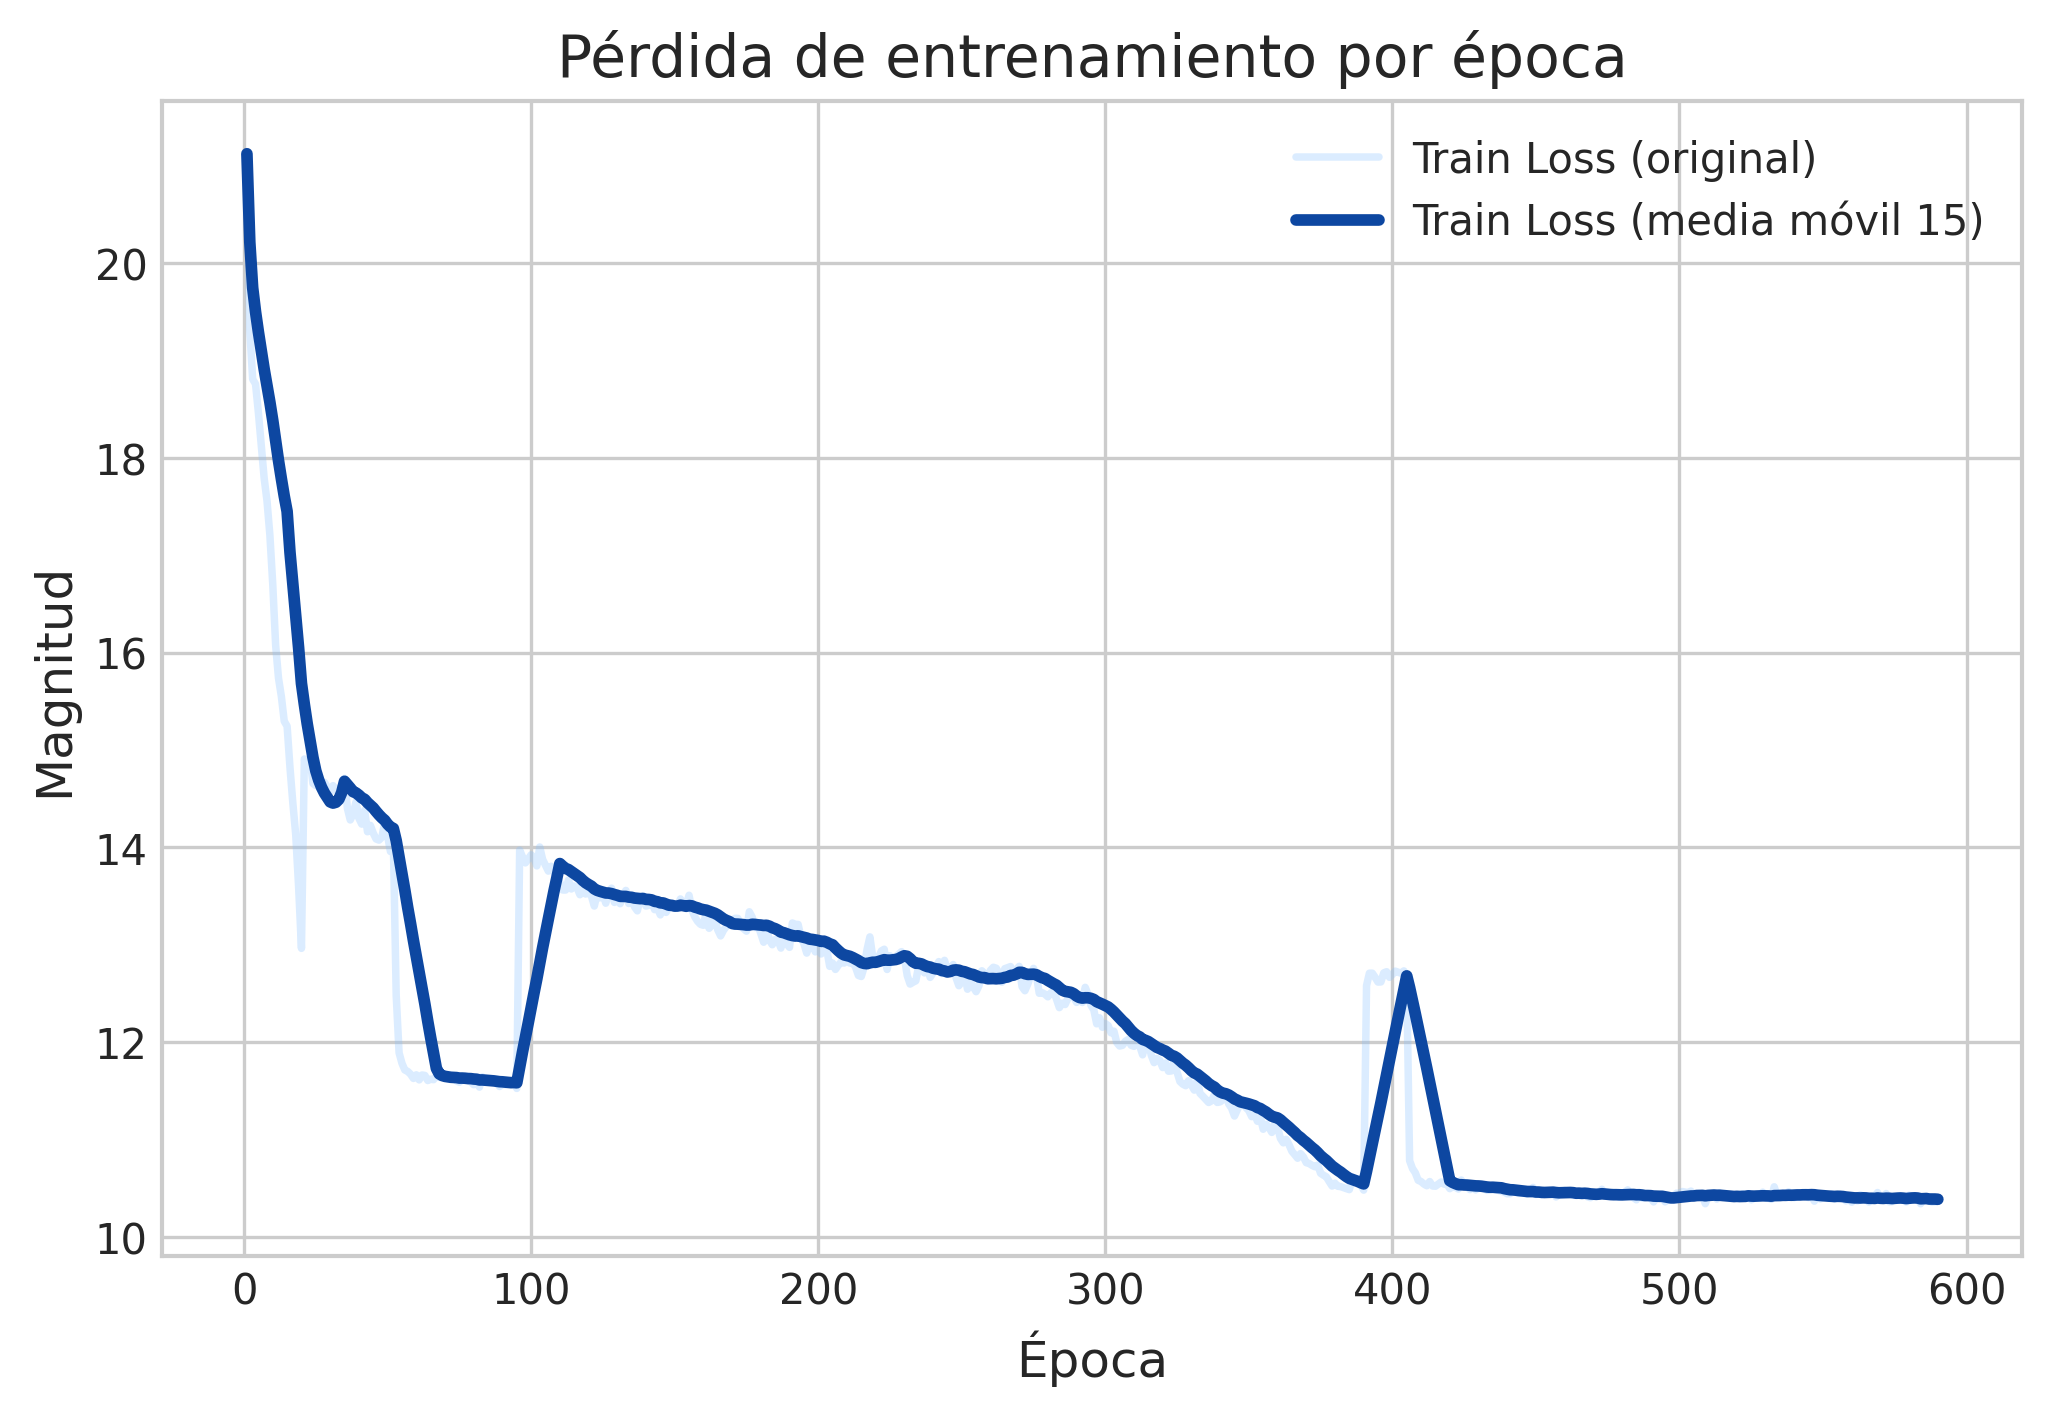
\includegraphics[width=0.48\textwidth]{../Figures/train_loss.png}
\hfill
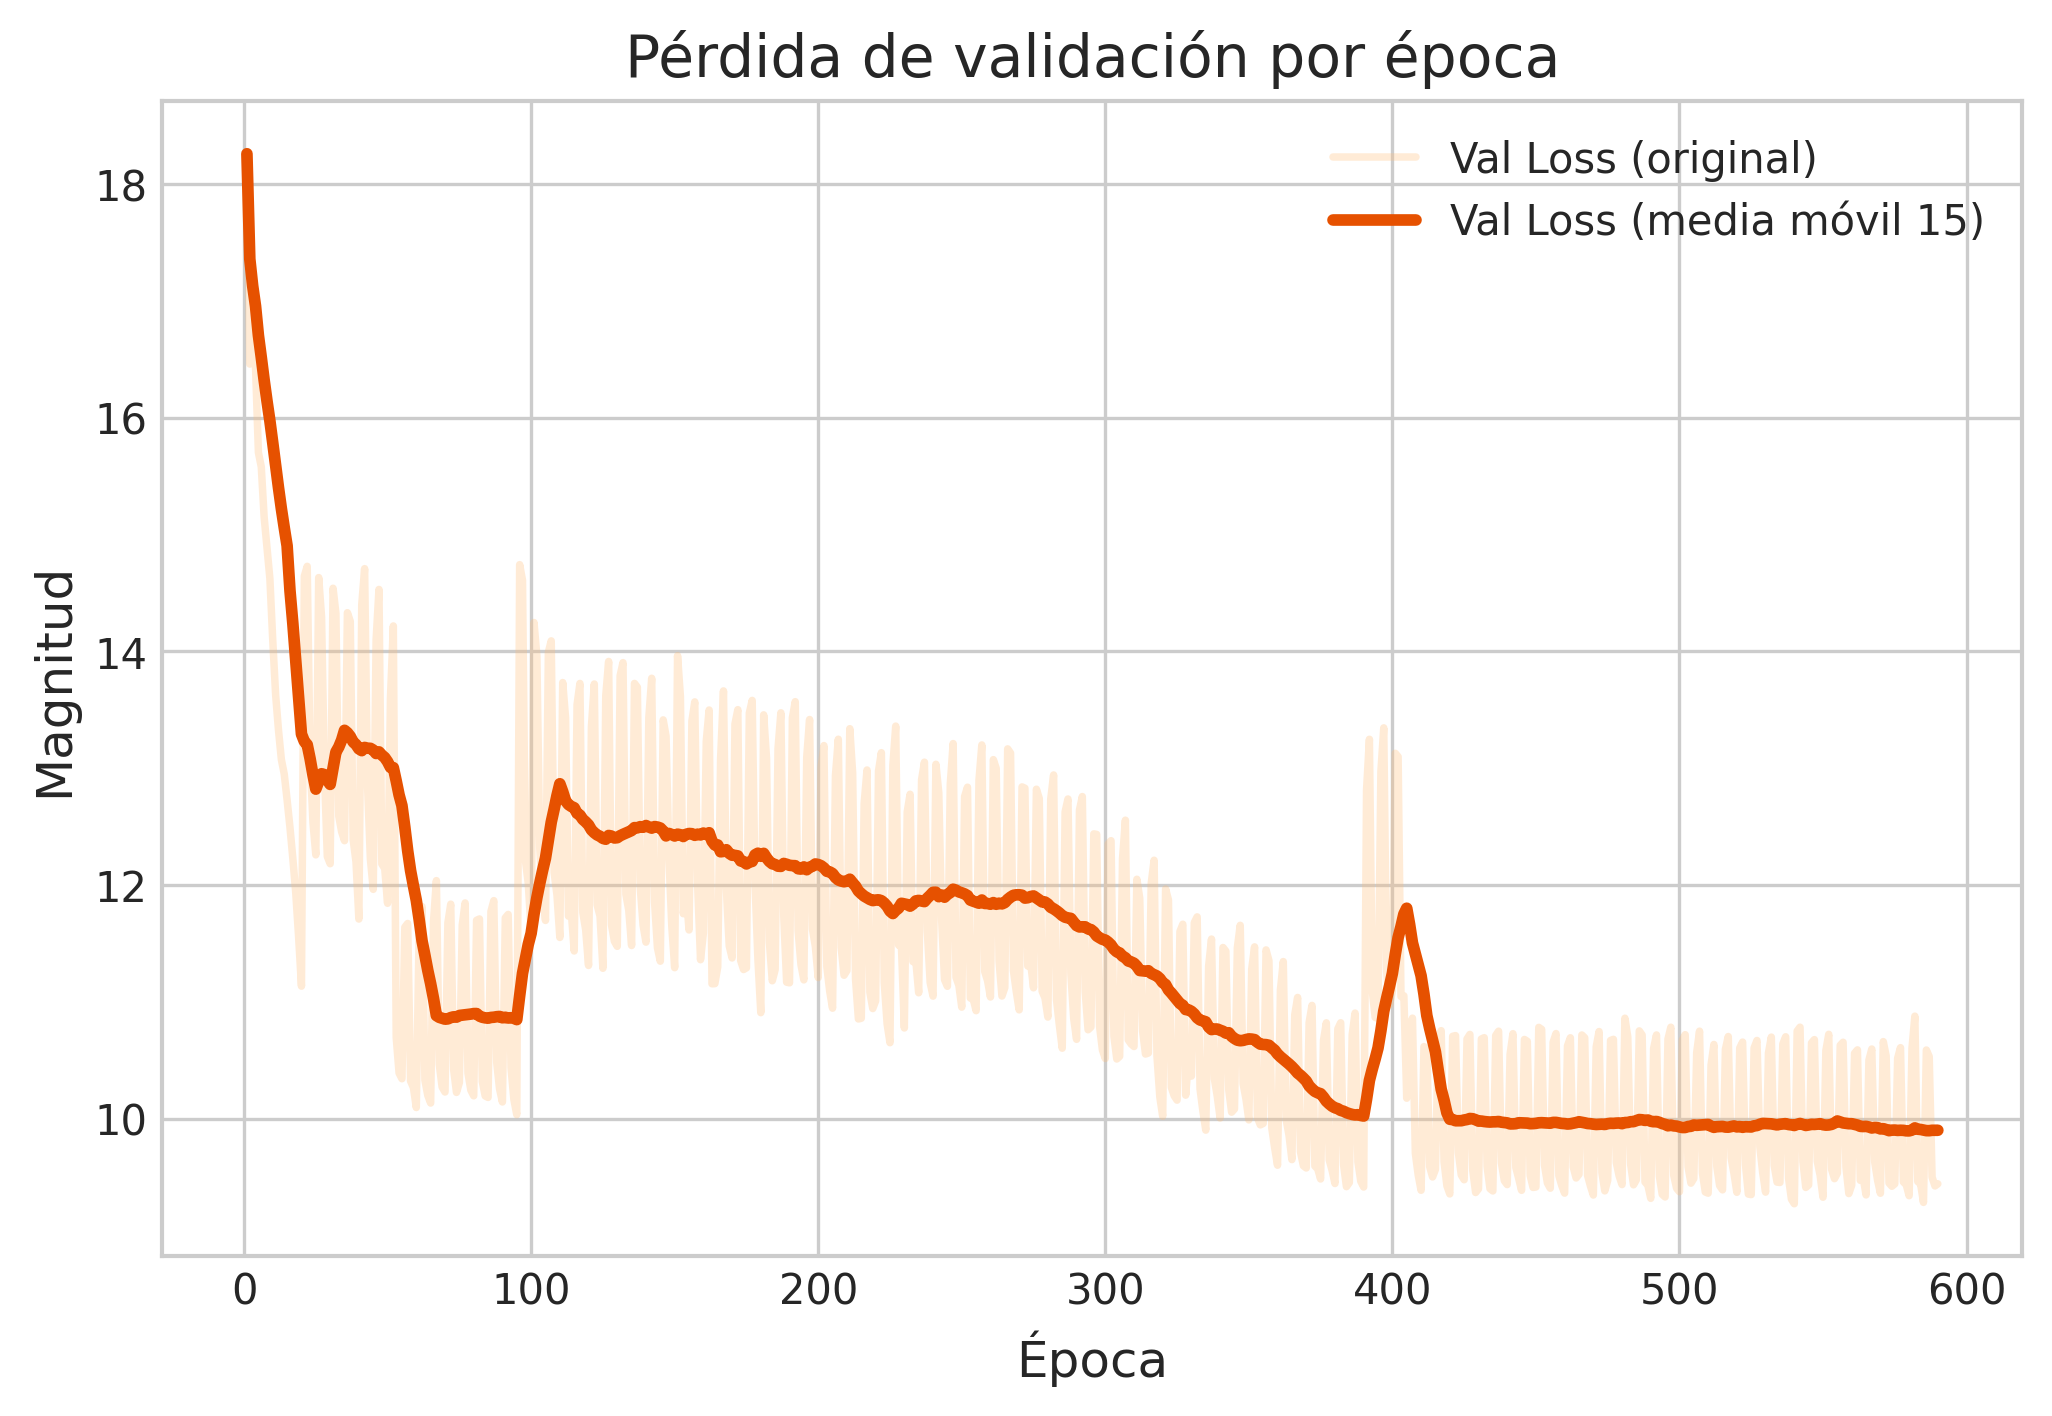
\includegraphics[width=0.48\textwidth]{../Figures/val_loss.png}
\caption{Evolución de la pérdida compuesta de entrenamiento y validación. Se superpone la tendencia suavizada mediante media móvil.}
\label{fig:loss_curves}
\end{figure}

La métrica física principal, definida como error absoluto medio sobre la Curva de Decaimiento de Energía (EDC-L1), presenta convergencia robusta durante el entrenamiento. En particular, la trayectoria perfora el umbral de 0.10 y se consolida en torno a 0.08 en las épocas finales, tal como se observa en la Figura~\ref{fig:edc_curves}. Este comportamiento confirma que la red no solo reduce error espectral, sino que también preserva la dinámica energética del decaimiento reverberante con precisión físicamente consistente.

\begin{figure}[htbp]
\centering
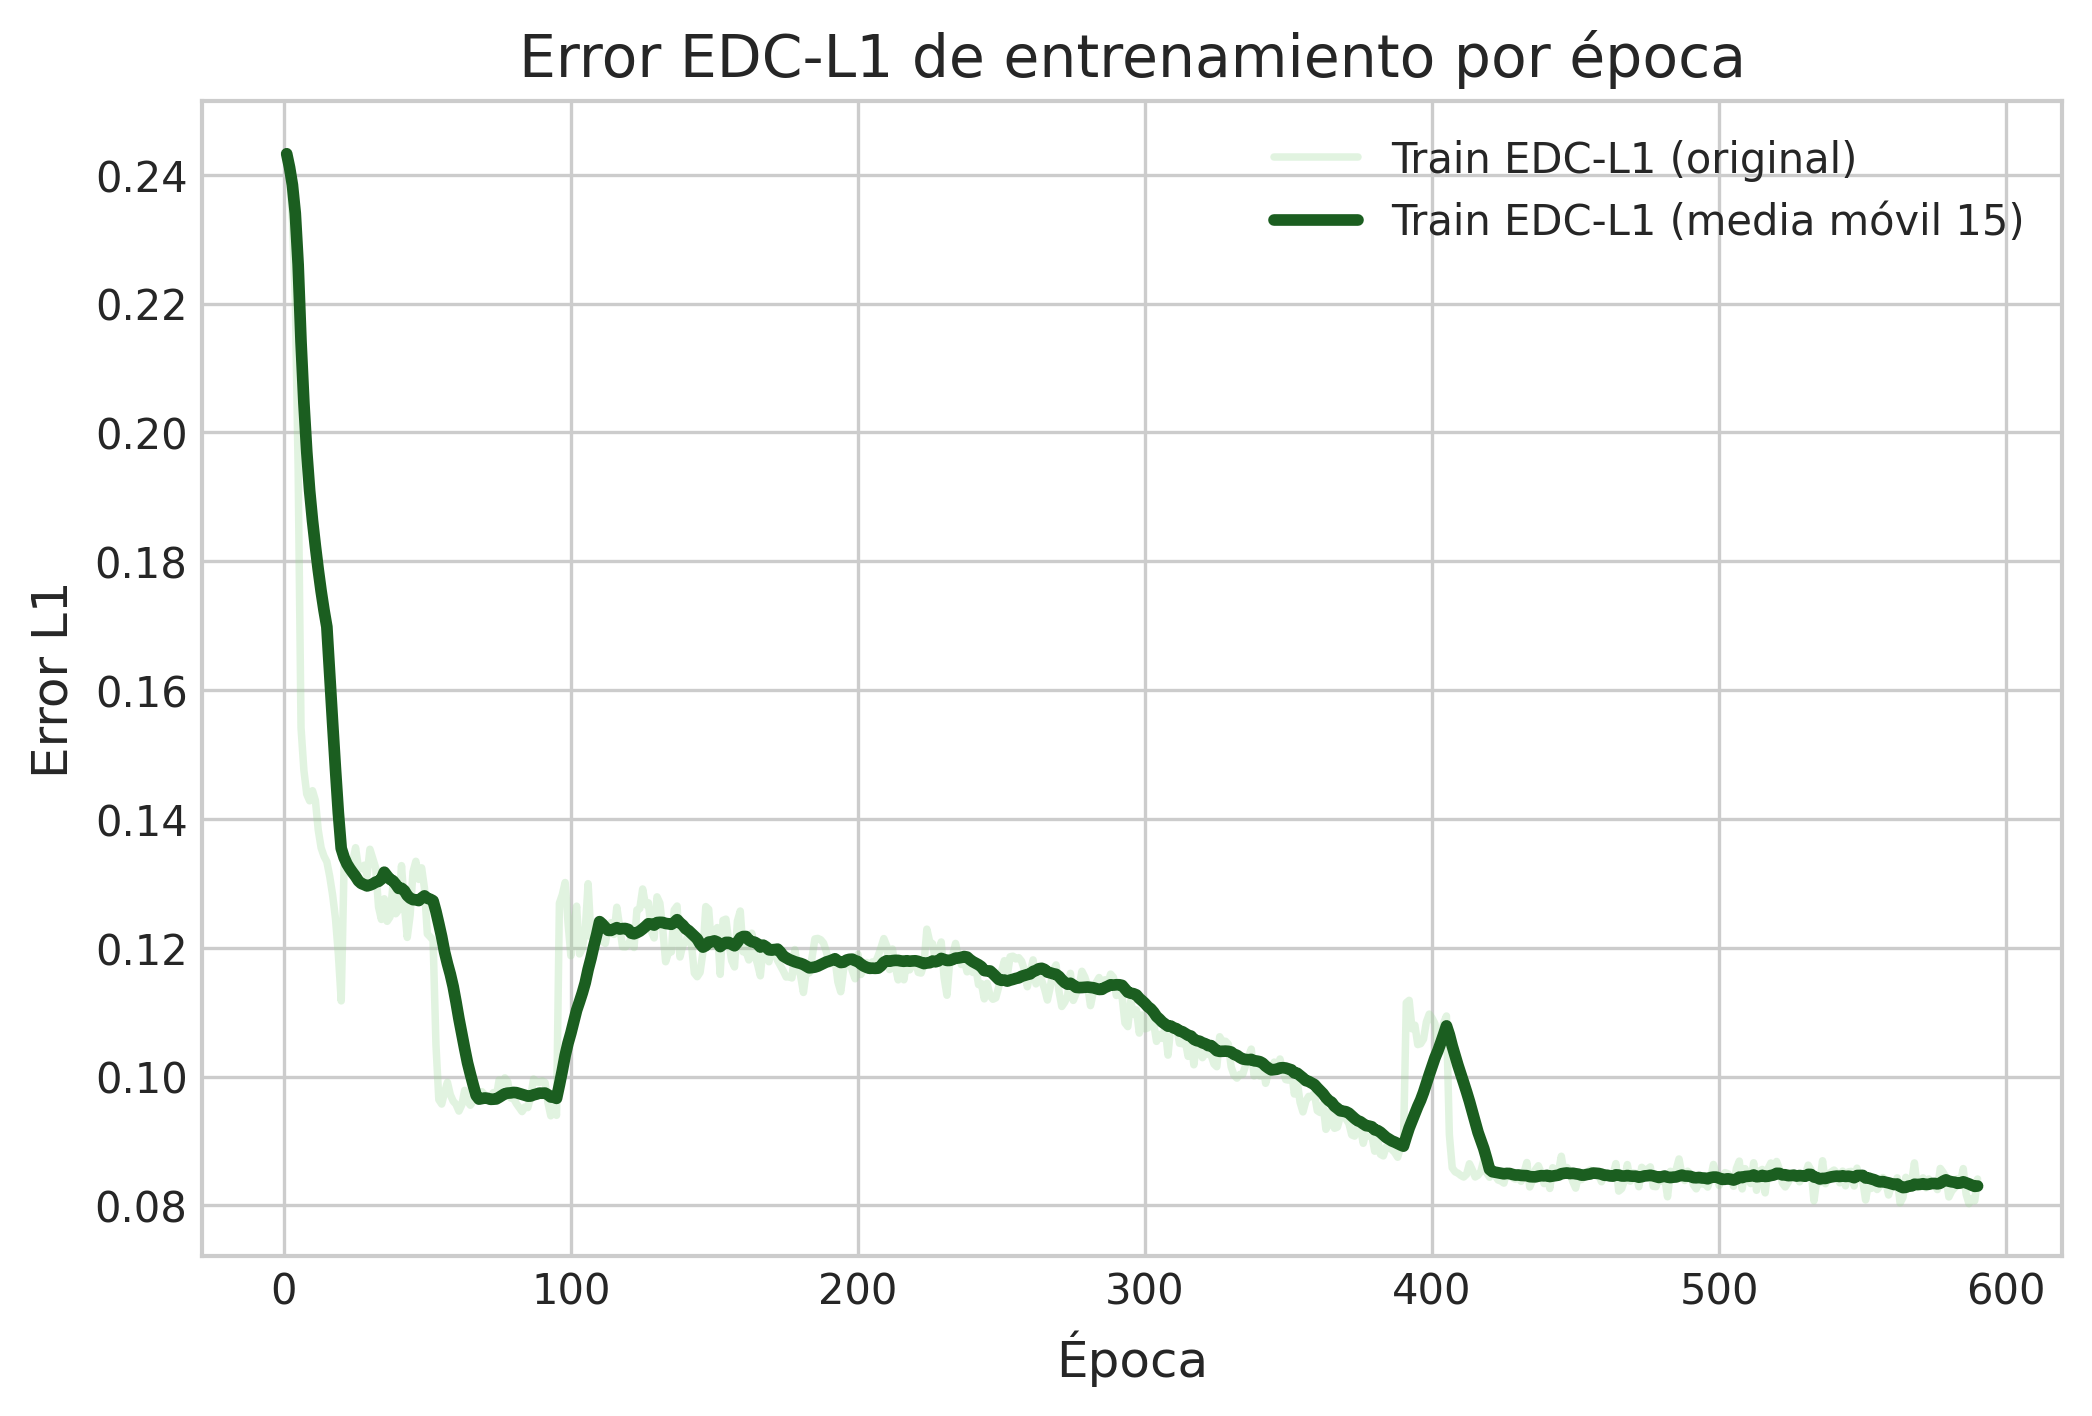
\includegraphics[width=0.48\textwidth]{../Figures/train_edc.png}
\hfill
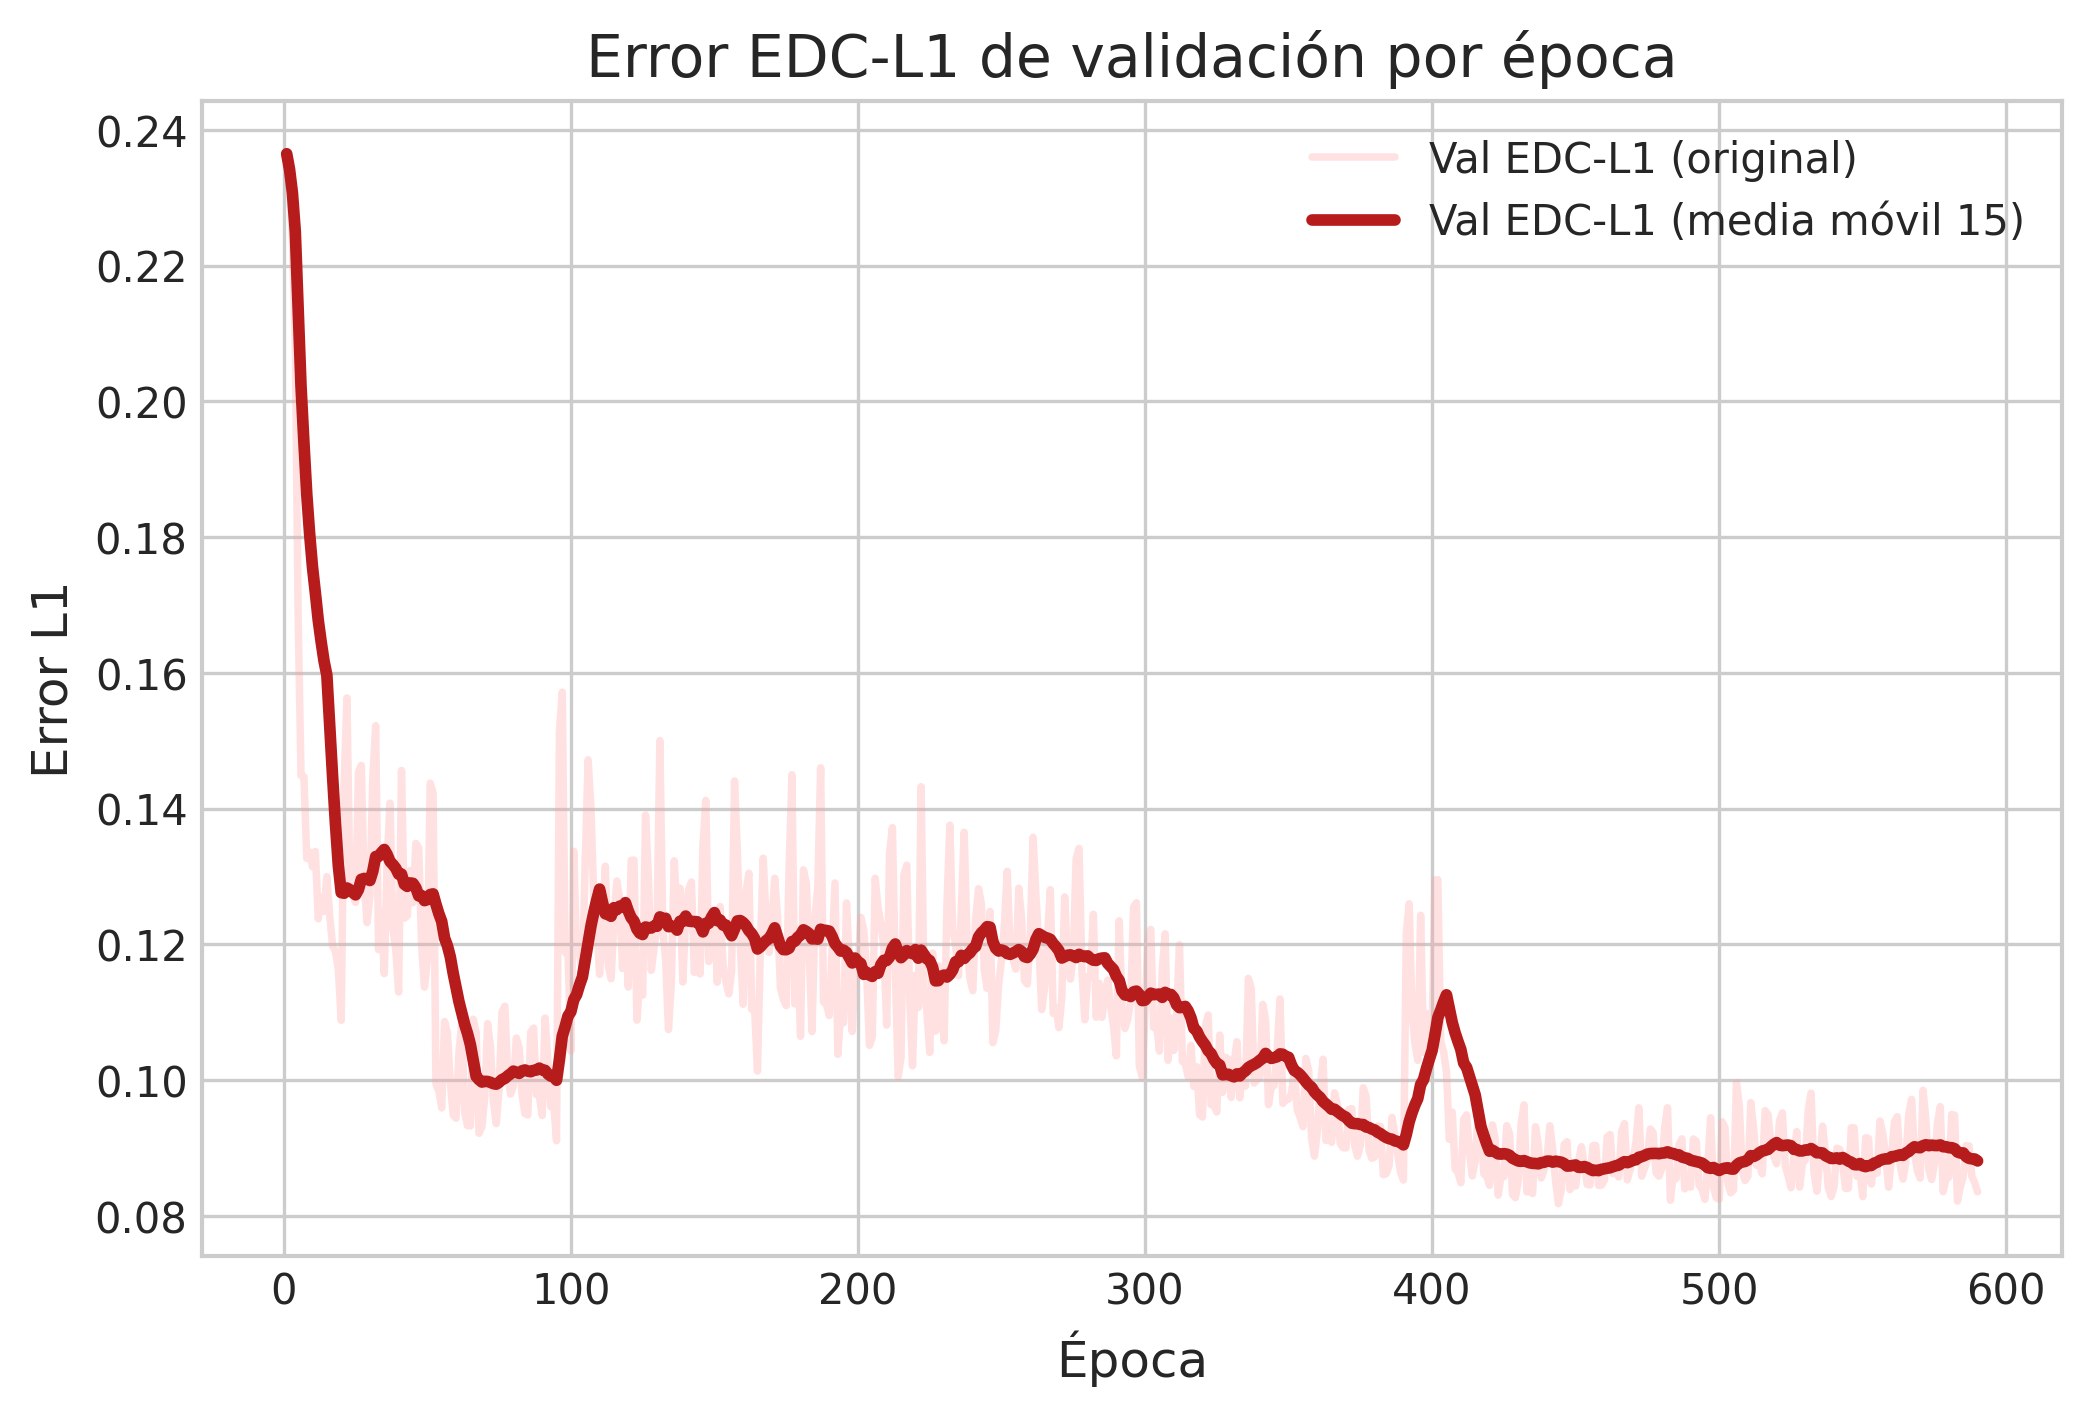
\includegraphics[width=0.48\textwidth]{../Figures/val_edc.png}
\caption{Convergencia del error absoluto medio de la Curva de Decaimiento de Energía (EDC-L1).}
\label{fig:edc_curves}
\end{figure}

Desde la perspectiva de estabilidad numérica, la predicción de tasas de decaimiento exponencial $b_k$ en el decodificador induce una superficie de pérdida fuertemente no convexa. La monitorización de la norma del gradiente, representada en la Figura~\ref{fig:gnorm}, evidencia picos transitorios severos que superan magnitudes del orden de $10^{4}$. Esta observación empírica justifica con rigor la necesidad técnica de emplear recorte de gradientes (\textit{gradient clipping}) dentro de Ranger21, mecanismo que resultó determinante para absorber inestabilidades locales y prevenir colapso numérico en los tensores durante fases críticas del aprendizaje.

\begin{figure}[htbp]
\centering
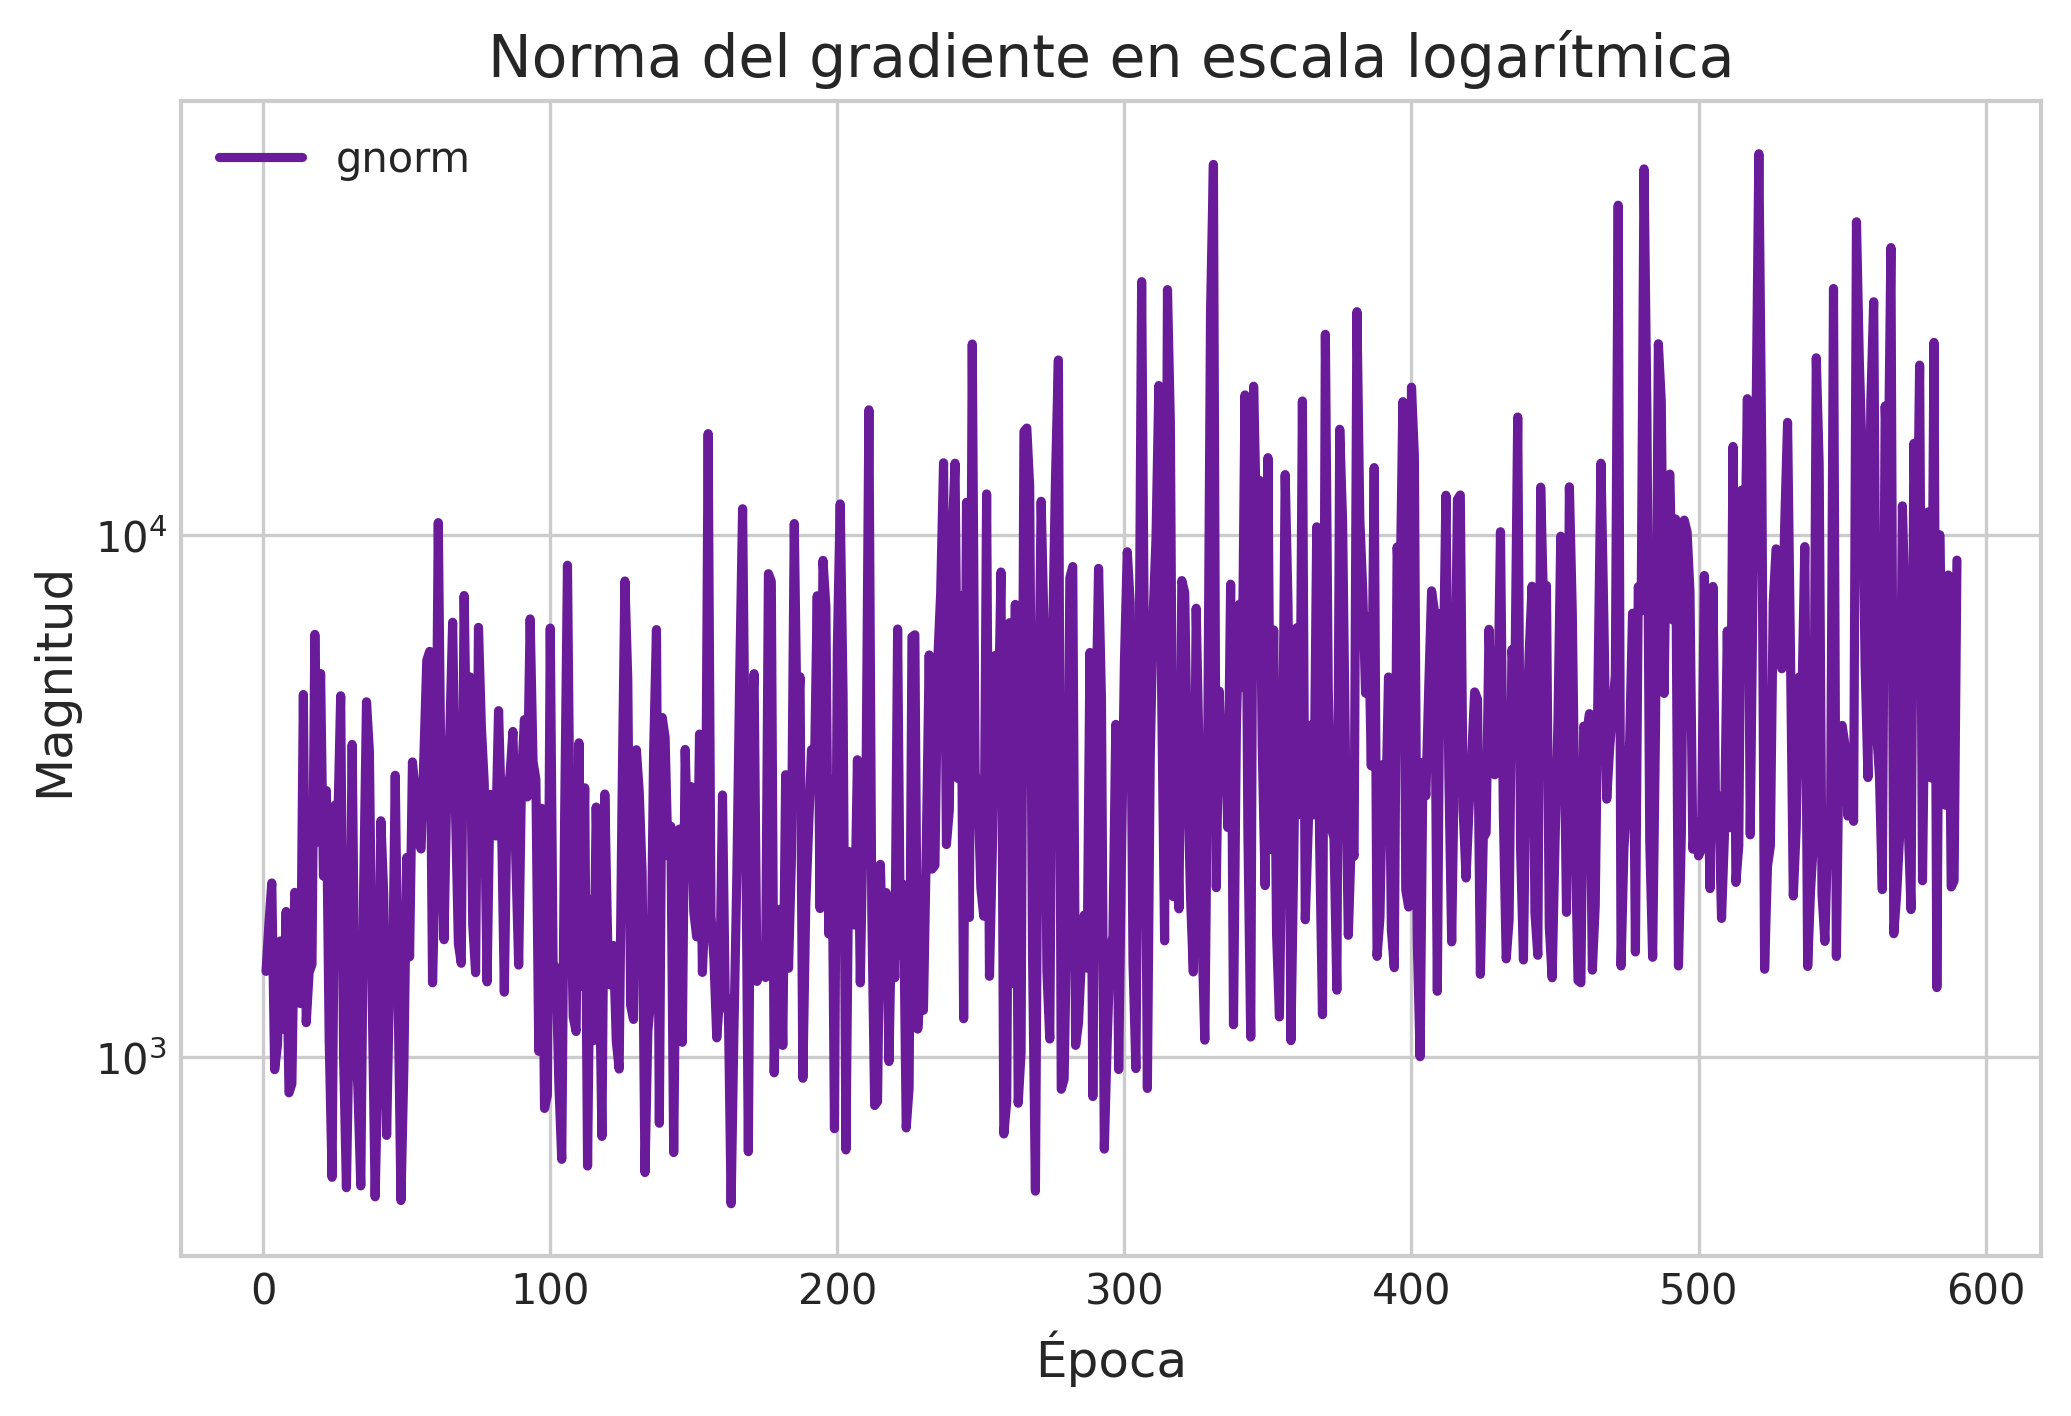
\includegraphics[width=0.75\textwidth]{../Figures/gnorm_log.png}
\caption{Evolución de la norma del gradiente en escala logarítmica durante el entrenamiento.}
\label{fig:gnorm}
\end{figure}

\section{Evaluación}

La validación cuantitativa del sistema se ha llevado a cabo sobre el subconjunto de test, compuesto por 40.000 muestras correspondientes a recintos no observados durante la fase de optimización. Para la inferencia se ha empleado el punto de control óptimo (\textit{checkpoint}) extraído en la época 540. El rendimiento se cuantifica mediante una doble perspectiva: por un lado, la fidelidad espectral global de la respuesta sintetizada y, por otro, la consistencia de descriptores acústicos físicos derivados de la Curva de Decaimiento de Energía (EDF).

\begin{lstlisting}[style=pythoncell,caption={Ejecución de la evaluación cuantitativa sobre el conjunto de test/validación.},label={lst:eval_run}]
CHECKPOINT_FINAL="/content/drive/MyDrive/TFG_Checkpoints/decor_v5_FINAL_ORO.pth"
DATA_LOCAL="/content/BIRD_Local"
python scripts/eval.py \
	--checkpoint "$CHECKPOINT_FINAL" \
	--data-root "$DATA_LOCAL"
\end{lstlisting}

\begin{table}[htbp]
\centering
\small
\setlength{\tabcolsep}{6pt}
\begin{tabular}{p{0.72\textwidth}r}
\toprule
\textbf{Métrica} & \textbf{Valor Medio ($\mu$)} \\
\midrule
Error Espectral Multiresolución (MSTFT) & 8.6108 \\
Error Absoluto Medio de la EDF (EDF MAE) [dB] & 5.39 \\
Raíz del Error Cuadrático Medio de la EDF (EDF RMSE) [dB] & 7.26 \\
Error Porcentual Absoluto Medio del $T_{60}$ ($T_{60}$ MAPE) [\%] & 8.1 \\
Error Cuadrático Medio de la Relación Directo-Reverberante (DRR MSE) [dB] & 7.24 \\
\bottomrule
\end{tabular}
\caption{Métricas de evaluación objetiva sobre el conjunto de test. Se reportan los valores medios obtenidos tras procesar las 40.000 muestras de evaluación.}
\label{tab:eval_objetiva}
\end{table}

Tal como se resume en la Tabla~\ref{tab:eval_objetiva}, el error MSTFT de 8.6108 cuantifica la fidelidad global de la distribución de energía espectrogramática y refleja una correspondencia robusta entre las envolventes espectro-temporales de referencia y las extrapoladas. De forma complementaria, los valores de EDF MAE (5.39 dB) y EDF RMSE (7.26 dB) evidencian un desajuste reducido en la pendiente de la cola reverberante en escala logarítmica, resultado que respalda una coherencia energética de alta precisión en la representación del decaimiento tardío.

En el plano de descriptores macroscópicos, el rendimiento alcanzado mantiene un nivel sobresaliente desde la perspectiva arquitectónica del sistema. El Error Porcentual Absoluto Medio del tiempo de reverberación, expresado como $T_{60}$ MAPE, se asienta en 8.1\%, y un margen confinado a un único dígito constituye evidencia empírica de que el decodificador infiere de forma correcta el volumen efectivo y la absorción equivalente de la sala. Finalmente, el DRR MSE de 7.24 dB constata la preservación del balance energético entre el campo acústico directo y el campo difuso, reforzando la validez física de las respuestas impulsionales reconstruidas.

La comparación con modelos de referencia, sintetizada en la Tabla~\ref{tab:comparativa_modelos}, permite situar el comportamiento del sistema en un marco competitivo. En dicha tabla, la métrica MSTFT se marca con flecha ascendente ($\uparrow$) para señalar de forma explícita que, en este contraste concreto, el valor del modelo propuesto resulta superior al de Naive y FiNS, es decir, no constituye su punto fuerte cuando se analiza únicamente el error espectral agregado. No obstante, el modelo propuesto exhibe mejoras sustanciales en los descriptores energéticos y macroscópicos de interés acústico, particularmente en EDF MAE, EDF RMSE, $T_{60}$ MAPE y DRR MSE. Este patrón respalda que la arquitectura está orientada a preservar con mayor fidelidad la estructura física del decaimiento reverberante y el balance energético global de la sala, objetivos centrales del presente trabajo.

\begin{table}[htbp]
\centering
\scriptsize
\setlength{\tabcolsep}{3pt}
\renewcommand{\arraystretch}{1.1}
\resizebox{0.98\textwidth}{!}{%
\begin{tabular}{lccccc}
\toprule
\textbf{Modelo} & \textbf{MSTFT ($\uparrow$)} & \textbf{EDF (MAE, dB, $\downarrow$)} & \textbf{EDF (RMSE, dB, $\downarrow$)} & \textbf{$T_{60}$ (MAPE, \%, $\downarrow$)} & \textbf{DRR (MSE, dB, $\downarrow$)} \\
\midrule
DECOR (propuesto) & 8.6108 & 5.39 & 7.26 & 8.1 & 7.24 \\
Naive & 3.53 & 12.8 & 17.3 & 41.6 & 14.5 \\
FiNS & 1.32 & 10.9 & 13.9 & 41.9 & 8.68 \\
\bottomrule
\end{tabular}%
}
\caption{Comparativa con modelos de referencia en métricas objetivas. En MSTFT se emplea flecha ascendente ($\uparrow$) para destacar que el valor del modelo propuesto es mayor que el de las referencias; en el resto de métricas, flecha descendente ($\downarrow$) indica mejor rendimiento para valores menores.}
\label{tab:comparativa_modelos}
\end{table}

\section{Caso cualitativo}

Con el propósito de interpretar el comportamiento del modelo más allá de las métricas numéricas agregadas, se examina cualitativamente un caso de estudio extraído del subconjunto de evaluación. Este análisis permite inspeccionar de forma directa la correspondencia entre señal de referencia y señal extrapolada en tres planos complementarios: la forma de onda temporal, la distribución espectro-temporal de energía y la dinámica de decaimiento energético acumulado.

\begin{figure}[htbp]
\centering
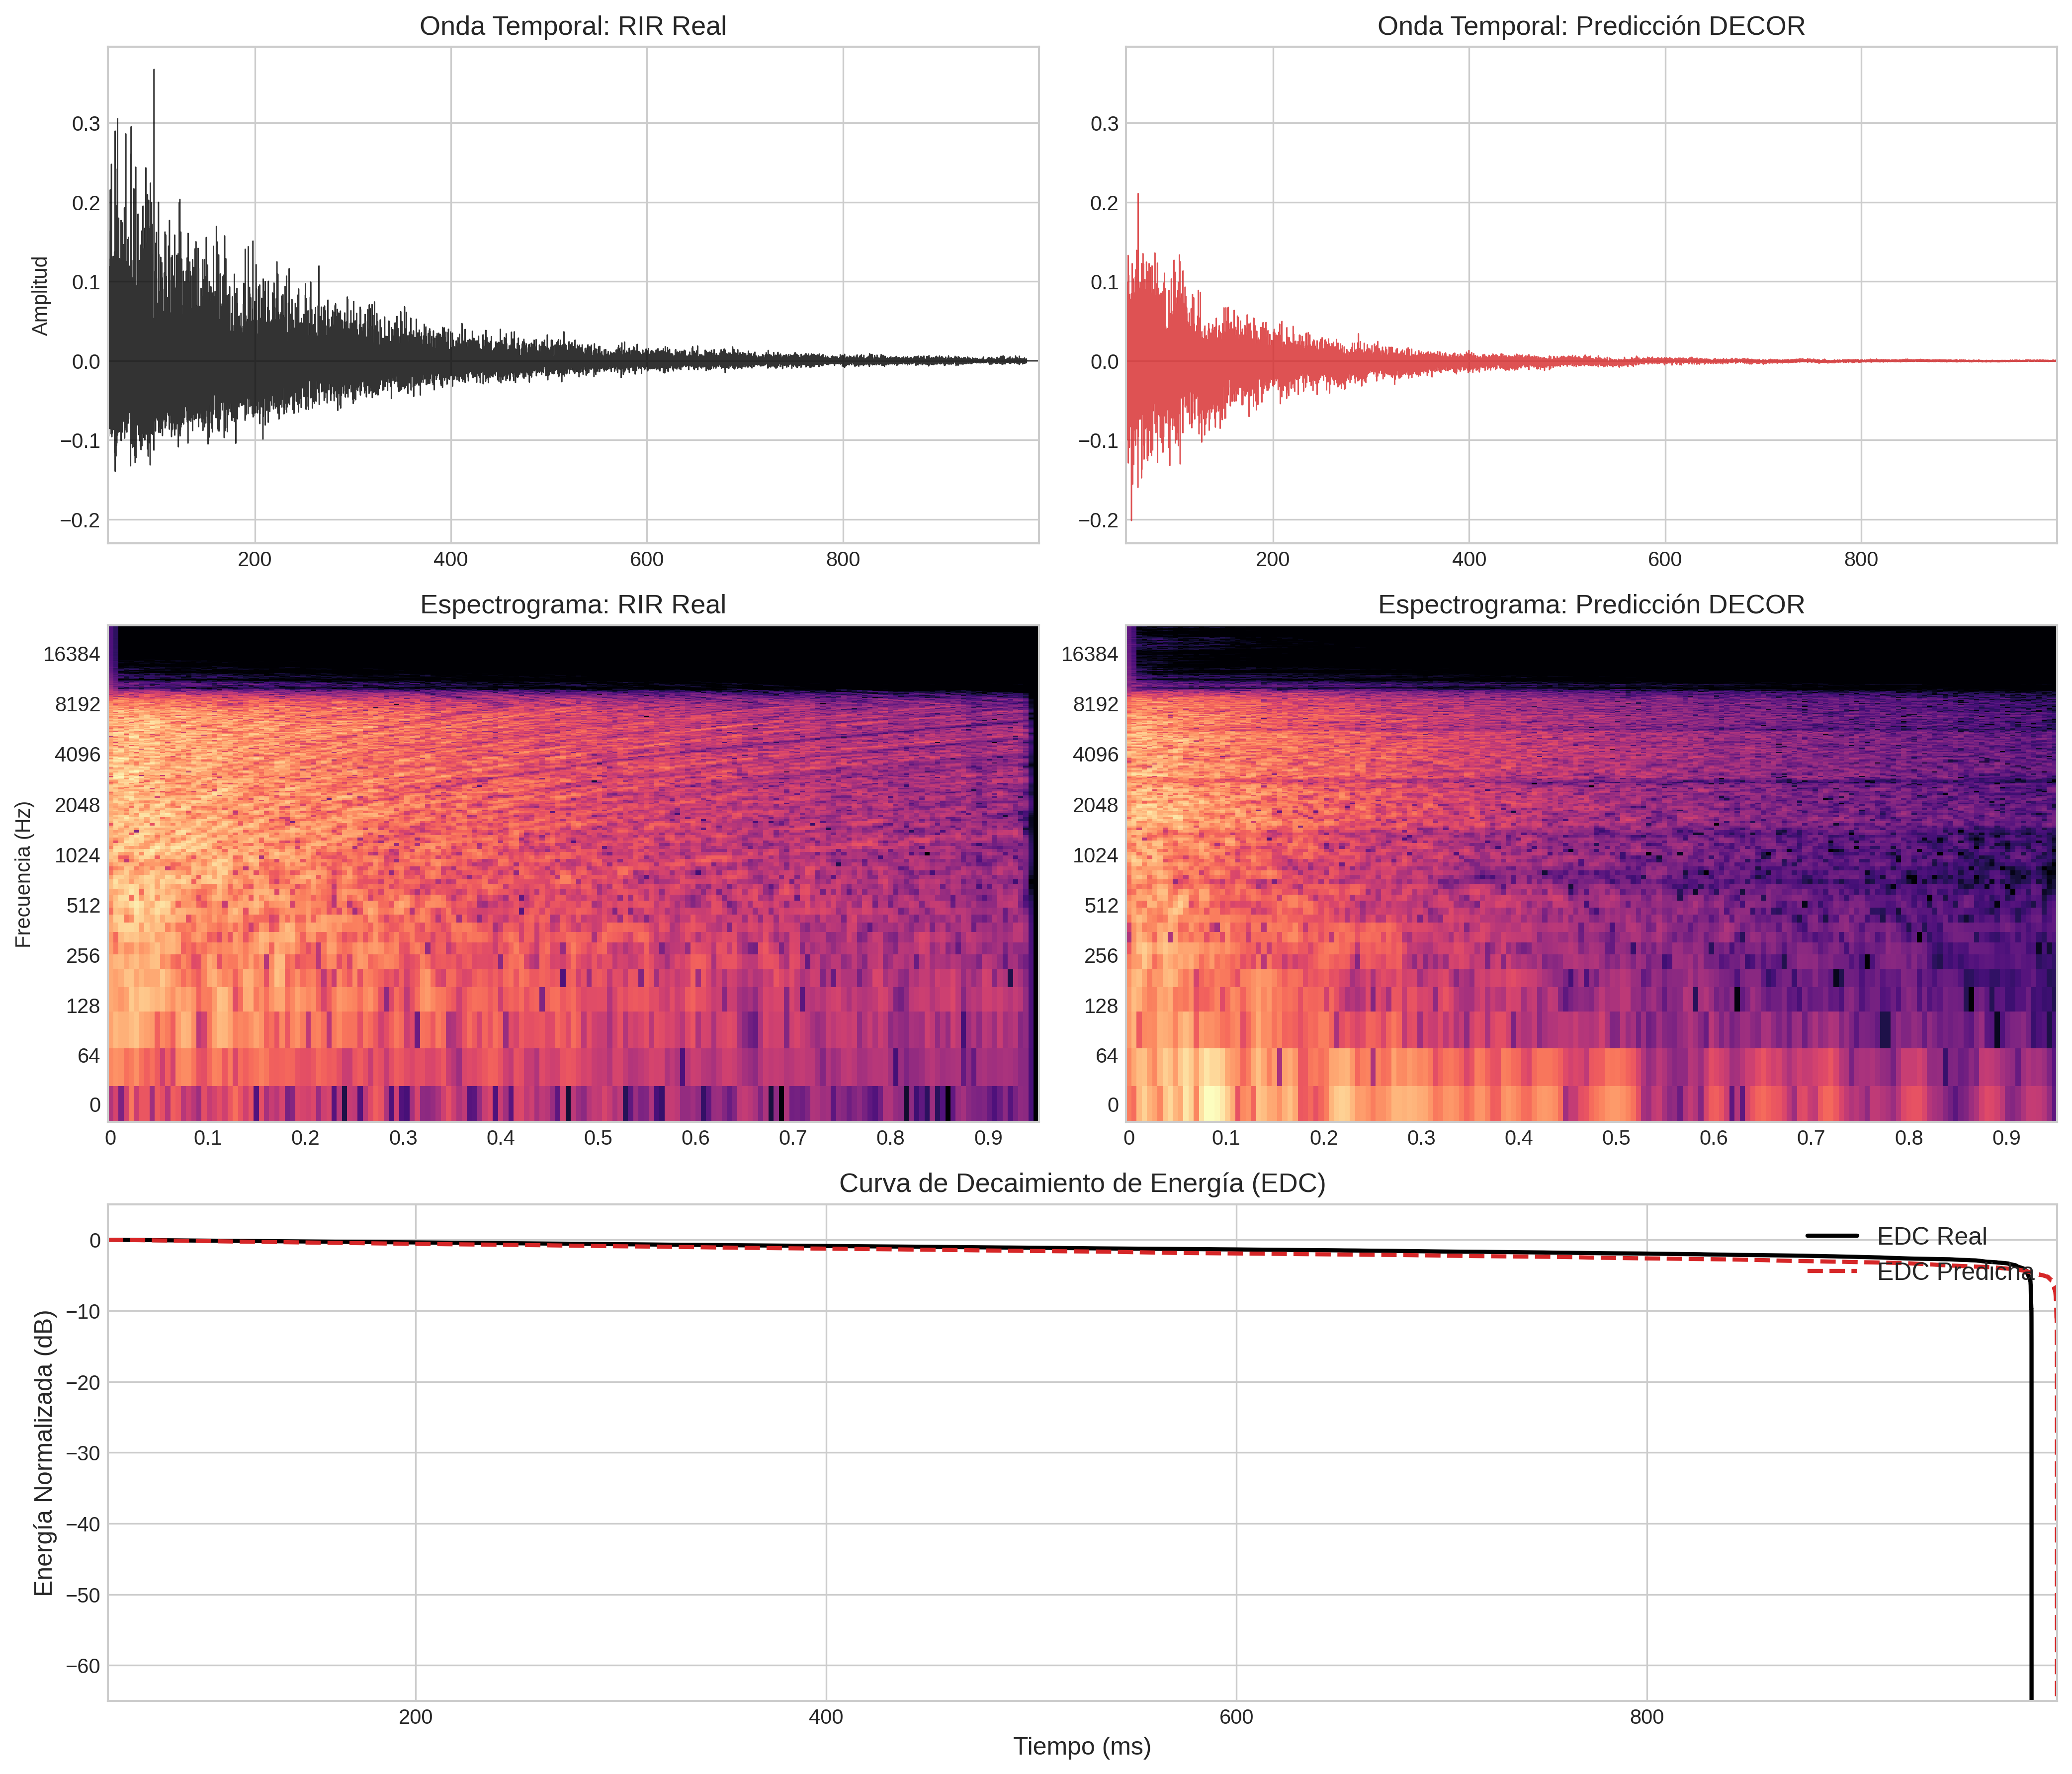
\includegraphics[width=1\textwidth]{../Figures/analisis_cualitativo.png}
\caption{Evaluación cualitativa de un caso de estudio. (Arriba) Comparativa de la forma de onda temporal. (Centro) Espectrogramas de magnitud. (Abajo) Curvas de Decaimiento de Energía (EDC).}
\label{fig:caso_estudio}
\end{figure}

Tal como se observa en la Figura~\ref{fig:caso_estudio}, la comparación de la forma de onda temporal puede sintetizarse en los siguientes puntos:

\textbf{Aciertos del modelo}
\begin{itemize}
\item \textbf{Envolvente de decaimiento.} DECOR reproduce con elevada fidelidad la estructura macro-temporal de la reverberación. La atenuación progresiva de la amplitud a lo largo del tiempo, asociada a la cola reverberante, resulta prácticamente coincidente con la respuesta real.
\item \textbf{Densidad de la cola reverberante.} A partir del régimen de campo difuso (aproximadamente desde 200 ms), la síntesis mantiene un patrón denso y estocástico coherente con la señal de referencia, convergiendo hacia niveles próximos a cero en un horizonte temporal equivalente.
\end{itemize}

\textbf{Puntos de mejora y limitaciones}
\begin{itemize}
\item \textbf{Subestimación de amplitud máxima.} La discrepancia más visible aparece en los picos iniciales: la señal real alcanza máximos superiores (del orden de 0.3), mientras que la señal estimada presenta picos más contenidos (en torno a 0.2), lo que equivale a una respuesta parcialmente atenuada en escala lineal.
\item \textbf{Pérdida de estructura fina en reflexiones tempranas.} En el intervalo inicial (aproximadamente 0--100 ms), la respuesta real presenta reflexiones tempranas discretas y bien separadas. La predicción conserva su localización global, pero las representa con mayor aglomeración y menor varianza local, reduciendo nitidez en el detalle microscópico de la onda.
\end{itemize}

En el dominio espectral, la lectura de la Figura~\ref{fig:caso_estudio} puede sintetizarse en los siguientes aspectos:

\textbf{Aciertos del modelo}
\begin{itemize}
\item \textbf{Envolvente macro y distribución de energía.} La predicción preserva la estructura global del espectrograma, reproduciendo con fidelidad tanto el impacto energético inicial como el decaimiento progresivo en el eje temporal.
\item \textbf{Decaimiento dependiente de la frecuencia.} Se mantiene un comportamiento físicamente coherente: las componentes de alta frecuencia se extinguen antes, mientras que las bandas bajas y medias conservan energía durante intervalos más prolongados.
\item \textbf{Alineación temporal del decaimiento.} El instante de agotamiento energético global se sitúa en un entorno temporal concordante con la referencia, lo que respalda una estimación consistente del tiempo reverberante efectivo.
\end{itemize}

\textbf{Puntos de mejora y limitaciones}
\begin{itemize}
\item \textbf{Efecto de suavizado.} La síntesis presenta una textura más difuminada que la señal medida, cuya microestructura estocástica resulta más rugosa en la cola tardía.
\item \textbf{Resolución modal en bajas frecuencias.} En la banda baja (aproximadamente 0--128 Hz), las trazas modales verticales se representan con menor nitidez y mayor cuantización espacial.
\item \textbf{Atenuación del fondo residual.} En el tramo final del decaimiento, la predicción tiende a suprimir con mayor intensidad el ruido de fondo tenue observado en la referencia.
\end{itemize}

La comparación de las curvas EDC, igualmente visible en la Figura~\ref{fig:caso_estudio}, puede resumirse del siguiente modo:

\textbf{Aciertos del modelo}
\begin{itemize}
\item \textbf{Seguimiento de la tendencia global.} Durante la mayor parte del eje temporal, la curva estimada se superpone de forma casi idéntica a la curva de referencia, reflejando una estimación precisa de la distribución energética macroscópica.
\item \textbf{Estabilidad sin desviaciones sistémicas.} No se observan saltos espurios, oscilaciones anómalas ni desplazamientos persistentes de nivel entre trayectorias, lo que indica normalización energética robusta.
\end{itemize}

\textbf{Puntos de mejora y limitaciones}
\begin{itemize}
\item \textbf{Divergencia en el truncamiento final.} En el entorno previo a la caída abrupta al suelo de ruido, la predicción tiende a retener energía ligeramente más tiempo o a decaer de forma menos brusca que la referencia.
\item \textbf{Sensibilidad al ruido de fondo estocástico.} La estimación del instante exacto de corte en la cola final mantiene una dificultad intrínseca elevada en modelos neuronales aplicados a audio.
\end{itemize}

En conjunto, pese a las discrepancias localizadas en la microtextura espectral y en el truncamiento final, la coincidencia global de patrones respalda que el sistema asimila con elevada precisión la dinámica energética del recinto y confirma su robustez matemática en extrapolación ciega.


\newpage

\chapter{Conclusiones y Trabajo Futuro}

\section{Conclusiones}

El presente Trabajo de Fin de Grado ha resuelto de forma satisfactoria el problema de la extrapolación de la respuesta al impulso tardía a partir de una observación parcial de 50~ms. La evidencia experimental obtenida confirma que la información contenida en el tramo temprano, cuando se procesa mediante una arquitectura físicamente informada, resulta suficiente para reconstruir con consistencia la dinámica energética de la cola reverberante en recintos no observados durante el aprendizaje.

El balance crítico de resultados permite establecer una conclusión de fondo: la arquitectura paramétrica propuesta, DECOR, demuestra que el Procesamiento de Señal Diferenciable (DDSP) introduce un sesgo inductivo termodinámico esencial para el problema abordado. Aunque enfoques puramente generativos del estado del arte pueden optimizar con mayor facilidad distancias espectrales agregadas como MSTFT, su comportamiento evidencia limitaciones estructurales al representar magnitudes físicas del recinto. En contraste, alcanzar un error del 8.1\% en la estimación de $T_{60}$ y preservar de manera robusta la Curva de Decaimiento de Energía (EDC) valida la hipótesis central del proyecto: en extrapolación de reverberación tardía, la coherencia acústica constituye un criterio de mayor relevancia que la similitud espectrogramática cruda.

Desde una perspectiva metodológica, también se han consolidado aportaciones de carácter transversal. La estabilización de gradientes mediante técnicas de recorte (\textit{gradient clipping}), junto con una estrategia de aprendizaje por currículo, resultó determinante para alcanzar convergencia en una superficie de pérdida marcadamente no convexa. Esta combinación permitió absorber transitorios de alta inestabilidad durante las fases de acoplamiento físico de la función de coste y condujo a un régimen final de optimización estable, reproducible y físicamente interpretable.

\section{Trabajo futuro}

Como primera línea de investigación, se propone abordar de forma explícita la síntesis de microestructura estocástica de la cola reverberante, aspecto donde el análisis cualitativo ha identificado limitaciones en factor de cresta y rugosidad fina. Una vía prometedora consiste en acoplar modelos generativos complementarios, tales como Redes Adversarias Generativas o Modelos de Difusión, condicionados por los parámetros físicos estimados por el bloque DDSP. Este esquema híbrido permitiría recuperar detalle microscópico sin comprometer la envolvente macroscópica ni la consistencia energética global.

De forma complementaria, se considera especialmente relevante explorar la extrapolación directa mediante arquitecturas Transformer. Su mecanismo de autoatención podría capturar dependencias temporales de largo alcance entre reflexiones tempranas y cola reverberante, permitiendo modelar con mayor flexibilidad la evolución espectro-temporal sin perder coherencia física cuando se incorporen restricciones acústicas en la función objetivo.

Una segunda línea prioritaria se orienta a la expansión espacial y multicanal del marco actual. En particular, la adaptación a representaciones inmersivas tridimensionales, como Ambisonics o formulaciones basadas en HRTF, abriría la posibilidad de extrapolar no solo la evolución temporal de la energía, sino también la direccionalidad del campo difuso. Esta extensión incrementaría de forma sustancial el alcance aplicado del método en escenarios de Realidad Virtual, auralización interactiva y reproducción espacial avanzada.

Finalmente, se propone profundizar en la optimización de inferencia con el objetivo de viabilizar su despliegue en tiempo real. Entre las estrategias más relevantes se encuentran la destilación del modelo hacia arquitecturas de menor coste computacional y la traslación de componentes críticos a implementaciones de bajo nivel. Este esfuerzo permitiría aproximar el uso de DECOR a plataformas embebidas y sistemas con restricciones estrictas de latencia, favoreciendo su transferencia efectiva a entornos de producción.


\newpage

\backmatter

\chapter{Presupuesto y viabilidad económica}

\section{Costes}

Para una estimación simple y coherente, se ha considerado un periodo de trabajo de febrero a junio (aprox. 21 semanas) con una dedicación media de 20 horas semanales del estudiante.

\textbf{Hipótesis utilizadas:}
\begin{itemize}
	\item Horas de estudiante: $21 \times 20 = 420$ h.
	\item Coste hora estudiante (ingeniero pre-júnior): 18 EUR/h.
	\item Dedicación de dirección académica (profesor): 40 h totales.
	\item Coste hora profesor (UPC Terrassa): 70 EUR/h.
	\item Google Colab Pro: 100 unidades informáticas con coste total de 10 EUR.
\end{itemize}

\begin{table}[htbp]
\centering
\caption{Resumen de costes del TFG (estimación simple)}
\begingroup
\small
\setlength{\tabcolsep}{4pt}
\begin{tabular}{p{5.2cm}rrr}
\toprule
\textbf{Concepto} & \textbf{Horas / unid.} & \textbf{Coste unitario} & \textbf{Coste total} \\
\midrule
Estudiante (ingeniero pre-júnior) & 420 h & 18 EUR/h & 7.560 EUR \\
Profesor (dirección y seguimiento) & 40 h & 70 EUR/h & 2.800 EUR \\
Google Colab Pro & 100 unidades informáticas & 0,10 EUR/unidad & 10 EUR \\
\midrule
\textbf{Total estimado} &  &  & \textbf{10.370 EUR} \\
\bottomrule
\end{tabular}
\endgroup
\end{table}

Esta estimación debe considerarse orientativa y sin impuestos indirectos, y resulta útil para valorar la viabilidad económica del desarrollo en un contexto académico.



\newpage

% !TeX root = ../main.tex

\chapter{Impacto ambiental y social}

El desarrollo de modelos de aprendizaje profundo para audio inmersivo no puede evaluarse de forma completa si se omite su dimensión energética. En el presente trabajo, el uso de aceleradores gráficos (GPU) de altas prestaciones ha sido una condición técnica necesaria para entrenar secuencias largas de señal acústica con estabilidad numérica y en tiempos razonables. Sin embargo, esta decisión metodológica conlleva un coste ambiental asociado al consumo eléctrico intensivo durante las fases de optimización.

Desde una perspectiva cuantitativa, la energía consumida durante entrenamiento puede aproximarse por

\begin{equation}
E \approx P_{med}\cdot T,
\end{equation}

donde $P_{med}$ representa la potencia media efectiva del sistema de cómputo y $T$ el tiempo total de uso. A su vez, la huella de carbono operativa puede estimarse como

\begin{equation}
\mathrm{CO_{2}eq} \approx E\cdot I_{red},
\end{equation}

siendo $I_{red}$ la intensidad de carbono de la red eléctrica que alimenta la infraestructura. Este marco evidencia que la eficiencia algorítmica no es únicamente una cuestión de rendimiento computacional, sino también un criterio de responsabilidad ambiental.

Bajo este enfoque, la arquitectura DECOR aporta una ventaja relevante: al introducir sesgo físico mediante DDSP y reducir dimensionalidad efectiva de la síntesis, permite alcanzar objetivos acústicos robustos con complejidad inferior a alternativas puramente generativas de mayor escala. En términos prácticos, una reducción de parámetros, épocas efectivas o tiempo de convergencia se traduce en menor demanda energética por experimento y, por extensión, en menor impacto ambiental acumulado en ciclos iterativos de investigación.

La reflexión social del proyecto se articula en dos planos. Primero, en el plano de acceso tecnológico, el alto coste de entrenamiento sobre GPU de gama alta puede ampliar la brecha entre grupos con distinta capacidad de cómputo. En consecuencia, el diseño de modelos más eficientes constituye también una estrategia de democratización científica. Segundo, en el plano aplicado, la capacidad de extrapolar reverberación realista con menor coste abre oportunidades en educación, accesibilidad y producción audiovisual, al facilitar herramientas acústicas avanzadas en contextos con recursos limitados.

Como criterio de buena práctica, se propone consolidar en trabajos futuros una política de cómputo responsable: monitorización explícita de consumo energético por experimento, reutilización sistemática de \textit{checkpoints}, priorización de búsquedas de hiperparámetros de bajo coste y reporte transparente de métricas de eficiencia junto a las métricas de precisión acústica. Este enfoque permite alinear rigor científico, sostenibilidad ambiental e impacto social positivo en el desarrollo de sistemas de inteligencia artificial para acústica computacional.

\newpage


\newpage
\printbibliography[heading=bibintoc]


\end{document}
